\documentclass[12pt,a4paper]{uefrep}
%
% Note, if you are writing in Finnish, modify commented lines in this file and
% modify also report_app.tex if you have appendices.
%
\usepackage[english]{babel}  % If writing in Finnish, replace egnlish with finnish
\usepackage[T1]{fontenc}
\usepackage{cite,url}
\usepackage[dvips]{graphicx}
\usepackage[tbtags]{amsmath}
\usepackage{psfrag}
\usepackage{ae,aecompl}
\usepackage{color}
\usepackage{bookmark}
\usepackage[a-1b]{pdfx}
\usepackage{hyperref}
\usepackage{subcaption}
\usepackage{listings}
\usepackage{xcolor}
%\usepackage{float}
\usepackage{amsthm,amssymb}
\usepackage{tabularx}
\usepackage{longtable} % for table header multicolumn

\definecolor{dkgreen}{rgb}{0,0.6,0}
\definecolor{gray}{rgb}{0.5,0.5,0.5}
\definecolor{mauve}{rgb}{0.58,0,0.82}

\lstset{frame=tb,
  language=Python,
  aboveskip=3mm,
  belowskip=3mm,
  showstringspaces=false,
  columns=flexible,
  basicstyle=\footnotesize,
  numbers=none,
  numberstyle=\tiny\color{gray},
  keywordstyle=\color{blue},
  commentstyle=\color{dkgreen},
  stringstyle=\color{mauve},
  breaklines=true,
  breakatwhitespace=true,
  tabsize=3
}


% LET TESTING





\hypersetup{colorlinks=true,linkcolor=blue,citecolor=red,urlcolor=blue,breaklinks=true}
%
%
\pagestyle{plain}
\bibliographystyle{uefunsrt}
\setlength{\textheight}{20.7cm}
\setlength{\textwidth}{15.0cm}
\setlength{\hoffset}{-2mm}  % Because the location of left margin depends on the printer, adjust this so that the left margin is 32 mm.
%\setlenght{\voffset}{2mm} % If necessary, adjust the top margin to 45 mm with this parameter.
%
\renewcommand{\baselinestretch}{1.2}
\newcommand{\BibTeX}{{\textrm B\kern-.05em{\textsc i\kern-.025em b}\kern-.08em
    T\kern-.1667em\lower.7ex\hbox{E}\kern-.125emX}}
\newcommand{\sep}{;~}

\newenvironment{conditions}
  {\par\vspace{\abovedisplayskip}\noindent\begin{tabular}{>{$}l<{$} @{${}={}$} l}}
  {\end{tabular}\par\vspace{\belowdisplayskip}}




\usepackage{floatrow}
% Table float box with bottom caption, box width adjusted to content
\newfloatcommand{capbtabbox}{table}[][\FBwidth]

\usepackage[font=small,labelfont=bf,tableposition=top]{caption}

\DeclareCaptionLabelFormat{andtable}{#1~#2  \&  \tablename~\thetable}





\begin{document}


%% LET TEST

\makeatletter 
\let\c@table\c@figure
\let\c@lstlisting\c@figure
\makeatother


%
\pagenumbering{roman}
%
%%% Edit properly, pay special attention to names and dates.
%
\thispagestyle{empty}
%
%\\[1.5cm]
%
{\centering
%
{\huge\textbf{Estimating installation parameters of photovoltaic systems in northern latitudes by mathematical model fitting 
%\footnote{%
%\color{red} Remember to read the report writing instructions!
%(report\_writing\_instructions.pdf)} % Remove this footnote after reading the writing instructions ;)
}}\\[1.5cm]
%
% If the title is long for a one line, divide it to multiple lines, and use the \\[2mm] command to 
% add 2mm space between the lines.
%
{\huge \textit{Timo Salola}}
%
\vfill
%
%%% Insert here a figure if you like or remove these lines
%
%\begin{figure}[!h]
%\centering
%\includegraphics[width=11cm]{fpfig.eps}
%\end{figure}
%\vfill
%
{%
\renewcommand{\baselinestretch}{1.0}
%
\texttt{\large MSc Thesis\\[1mm] % or BSc thesis
August 2024\\
Department of Physics and Mathematics\\
University of Eastern Finland\\%
}}}
%
% This will create the frame for the front page.
%
\setlength{\unitlength}{1mm}
\linethickness{1.5pt}
\vspace{-25cm}
\begin{picture}(170,260)(13.5,-5)
% 
% For displays these picture settings in brackets above are fine, but for paper prints, the
% frame position may require some adjustment. If needed, adjust the last two parameters 
% so that when printed the frame is 25 mm from left and 25 mm from top of the page
%
\put(-5,-40.3){\line(1,0){170}}
\put(-5,225){\line(1,0){170}}
\put(-5,-40.6){\line(0,1){265.84}}
\put(165,-40.6){\line(0,1){265.84}}
\end{picture}\\


\newpage
\include{thesis_abs}
%
\newpage                     % (Un)comment these lines depending on if you have or not have a preface
\phantomsection
\hypertarget{prefacepage}{}
\bookmark[dest=prefacepage]{Preface}
%
\section*{\prefacename}
%Write the preface here. n the preface, you may inform the reader about your motivation to write your thesis and your experiences during the writing of your thesis. You can also use the preface to help the reader get started and to thank people who have helped you with your hesis.
As someone whose interests and strengths lie in geometry and programming, the real-world problem of panel installation parameter estimation was appealing from the beginning. I would like to thank William Wandji and Juha Karhu for their insights on the effects of clouds, snow and temperature on solar PV installation data. And Luna for being a supportive cat.

\vspace{3mm}
\noindent This research was funded by the Academy of Finland, decision 350695.


\vspace{9mm}
\noindent
Helsinki, the 20th of May 2024 %
%
%%% the signature below has some artistic freedom : )
%
\vspace{11mm}
\hspace{1.6cm}\emph{Timo Salola}

\vfill















     %
%
\phantomsection
\hypertarget{contentpage}{}
\bookmark[dest=contentpage]{Contents}
\tableofcontents
%
\newpage
\setcounter{page}{0}
\pagenumbering{arabic}
%

% ############################## INCLUDES HERE
\chapter{Introduction}

This thesis examines a specific applied mathematics problem suggested by the Finnish Meteorological institute FMI. The goal is to determine the geographic location and panel installation angles of photovoltaic solar power installations using only the power output data. The chosen method breaks down the problem of solving the geographic location and panel angles into separate algorithms. In practice, this means that the algorithms used can be less complex as they do not have to solve every unknown variable simultaneously, and visualizations of individual algorithms should also be more straightforward. Using multiple algorithms also splits the parameter space into smaller spaces, thus improving the performance of fitting algorithms. And the final benefit is the ability to focus on solving only the unknown parameters. For example, if the geolocation of a system is known and the panel installation angles are not, instead of estimating the geolocation, the known geolocation can be used for panel angle estimation, resulting in higher prediction accuracy.


The applications of parameter estimation algorithms would be in improving the quality of metadata in solar PV datasets. This could have implications for solar PV research, but the existence of such algorithms poses privacy and security-related questions as well. Whether these research benefits and concerns are realized depends on the accuracy, and to some extent, the ease of use of the algorithms.



A similar study was done by N. Haghdadi et al. in 2017\cite{navid_australian_article}. The 2017 article contains results from five case studies where the standard deviation of longitude prediction errors is less than $1.5^\circ$, reaching as low as $0.08^\circ$ with case study 1-2. The standard deviation of latitude predictions is higher at less than 3.5$^\circ$ with the best result in case study 2-2 with a standard deviation of 1.65$^\circ$. Azimuth and tilt predictions are reported as two separate angle error values with azimuth prediction errors reaching values between 4$^\circ$ and 27$^\circ$ and tilt 1.3$^\circ$ to 11.5$^\circ$. These forementioned results are not directly comparable to the results shown in this thesis due to different datasets, geographic location and local climate, but they provide some perspective.



Another article of relevance written by M.K. Williams et al. in 2012\cite{older_solar_solver_article} proposes multiple methods for determining the locations and orientations of solar PV installations. Perhaps the most interesting contribution of the 2012 article is the network approach to determining geographic location. This method relies on a grid of installations with known and accurate geolocation and installation angles. According to the authors, this networked approach works up to a 10-mile accuracy when the grid of known installations is dense around the estimated installation. This could make the network approach preferable for electric companies or institutions with large amounts of data. But as of now, it does not seem usable for FMI.

\chapter{Installations and datasets}

\noindent A simple PV installation consists of a solar panel or a set of solar panels, an inverter and optionally a battery system. Each of these components can be configured in several different ways and how this is done depends on how installation costs, maintenance, production peak consumption hours, total output and a multitude of other factors are balanced. This variability and difference in demands results in a large variance in PV systems, but some generalizations can still be made. A typical PV installation consists of a set of PV panels which are all installed at the same installation angles. In Finland such installations are typically installed on the roofs of offices or detached houses. As the panel angles in a such system are the same, the solar panels can be modeled as a single larger solar panel in most circumstances and this makes system modeling easier.


Less common but still worth noting are PV installations with mixed installation angles. In these, individual panels or sets of panels have different installation angles. This means that modeling a such system requires the use of multiple surfaces, increasing the model complexity. A typical motivation behind a such installation would be maximizing the available surface area on the roof of a detached house or evening the power output of a PV system through a day. In rare cases PV panels may also be installed on tracking mounts which adjust the panel angles in order to maximize the output of the PV system which further complicates modeling.

The two datasets used in this thesis are from FMI. First dataset is from an installation on top of the FMI office building in Kumpula, Helsinki and it consists of two sets of fixed angle solar panels with identical installation angles. One of these sets or strings is shown in figure \ref{fig_fmikumpula_panels} and a section of data gathered from this installation is shown in table \ref{table_fmi_kumpula_csv}. This data gathering is done by the inverter. The Kuopio installation is similar to the Helsinki installation in most respects with the most significant differences being the azimuth angle and different local climate. Shadowing also appears to be more common on the Kuopio installation. Parameters of the two installations are listed on table \ref{table_fmi_helsinki_kuopio_parameters}.




%The tilt angle of the panels in this figure appears to match the 15$^\circ$ tilt listed on table \ref{table_fmi_helsinki_kuopio_parameters}. The installation in Kuopio is similar in size and it also consists of two sets of panels with the same installation angles. 

\begin{figure}[h]
\centering
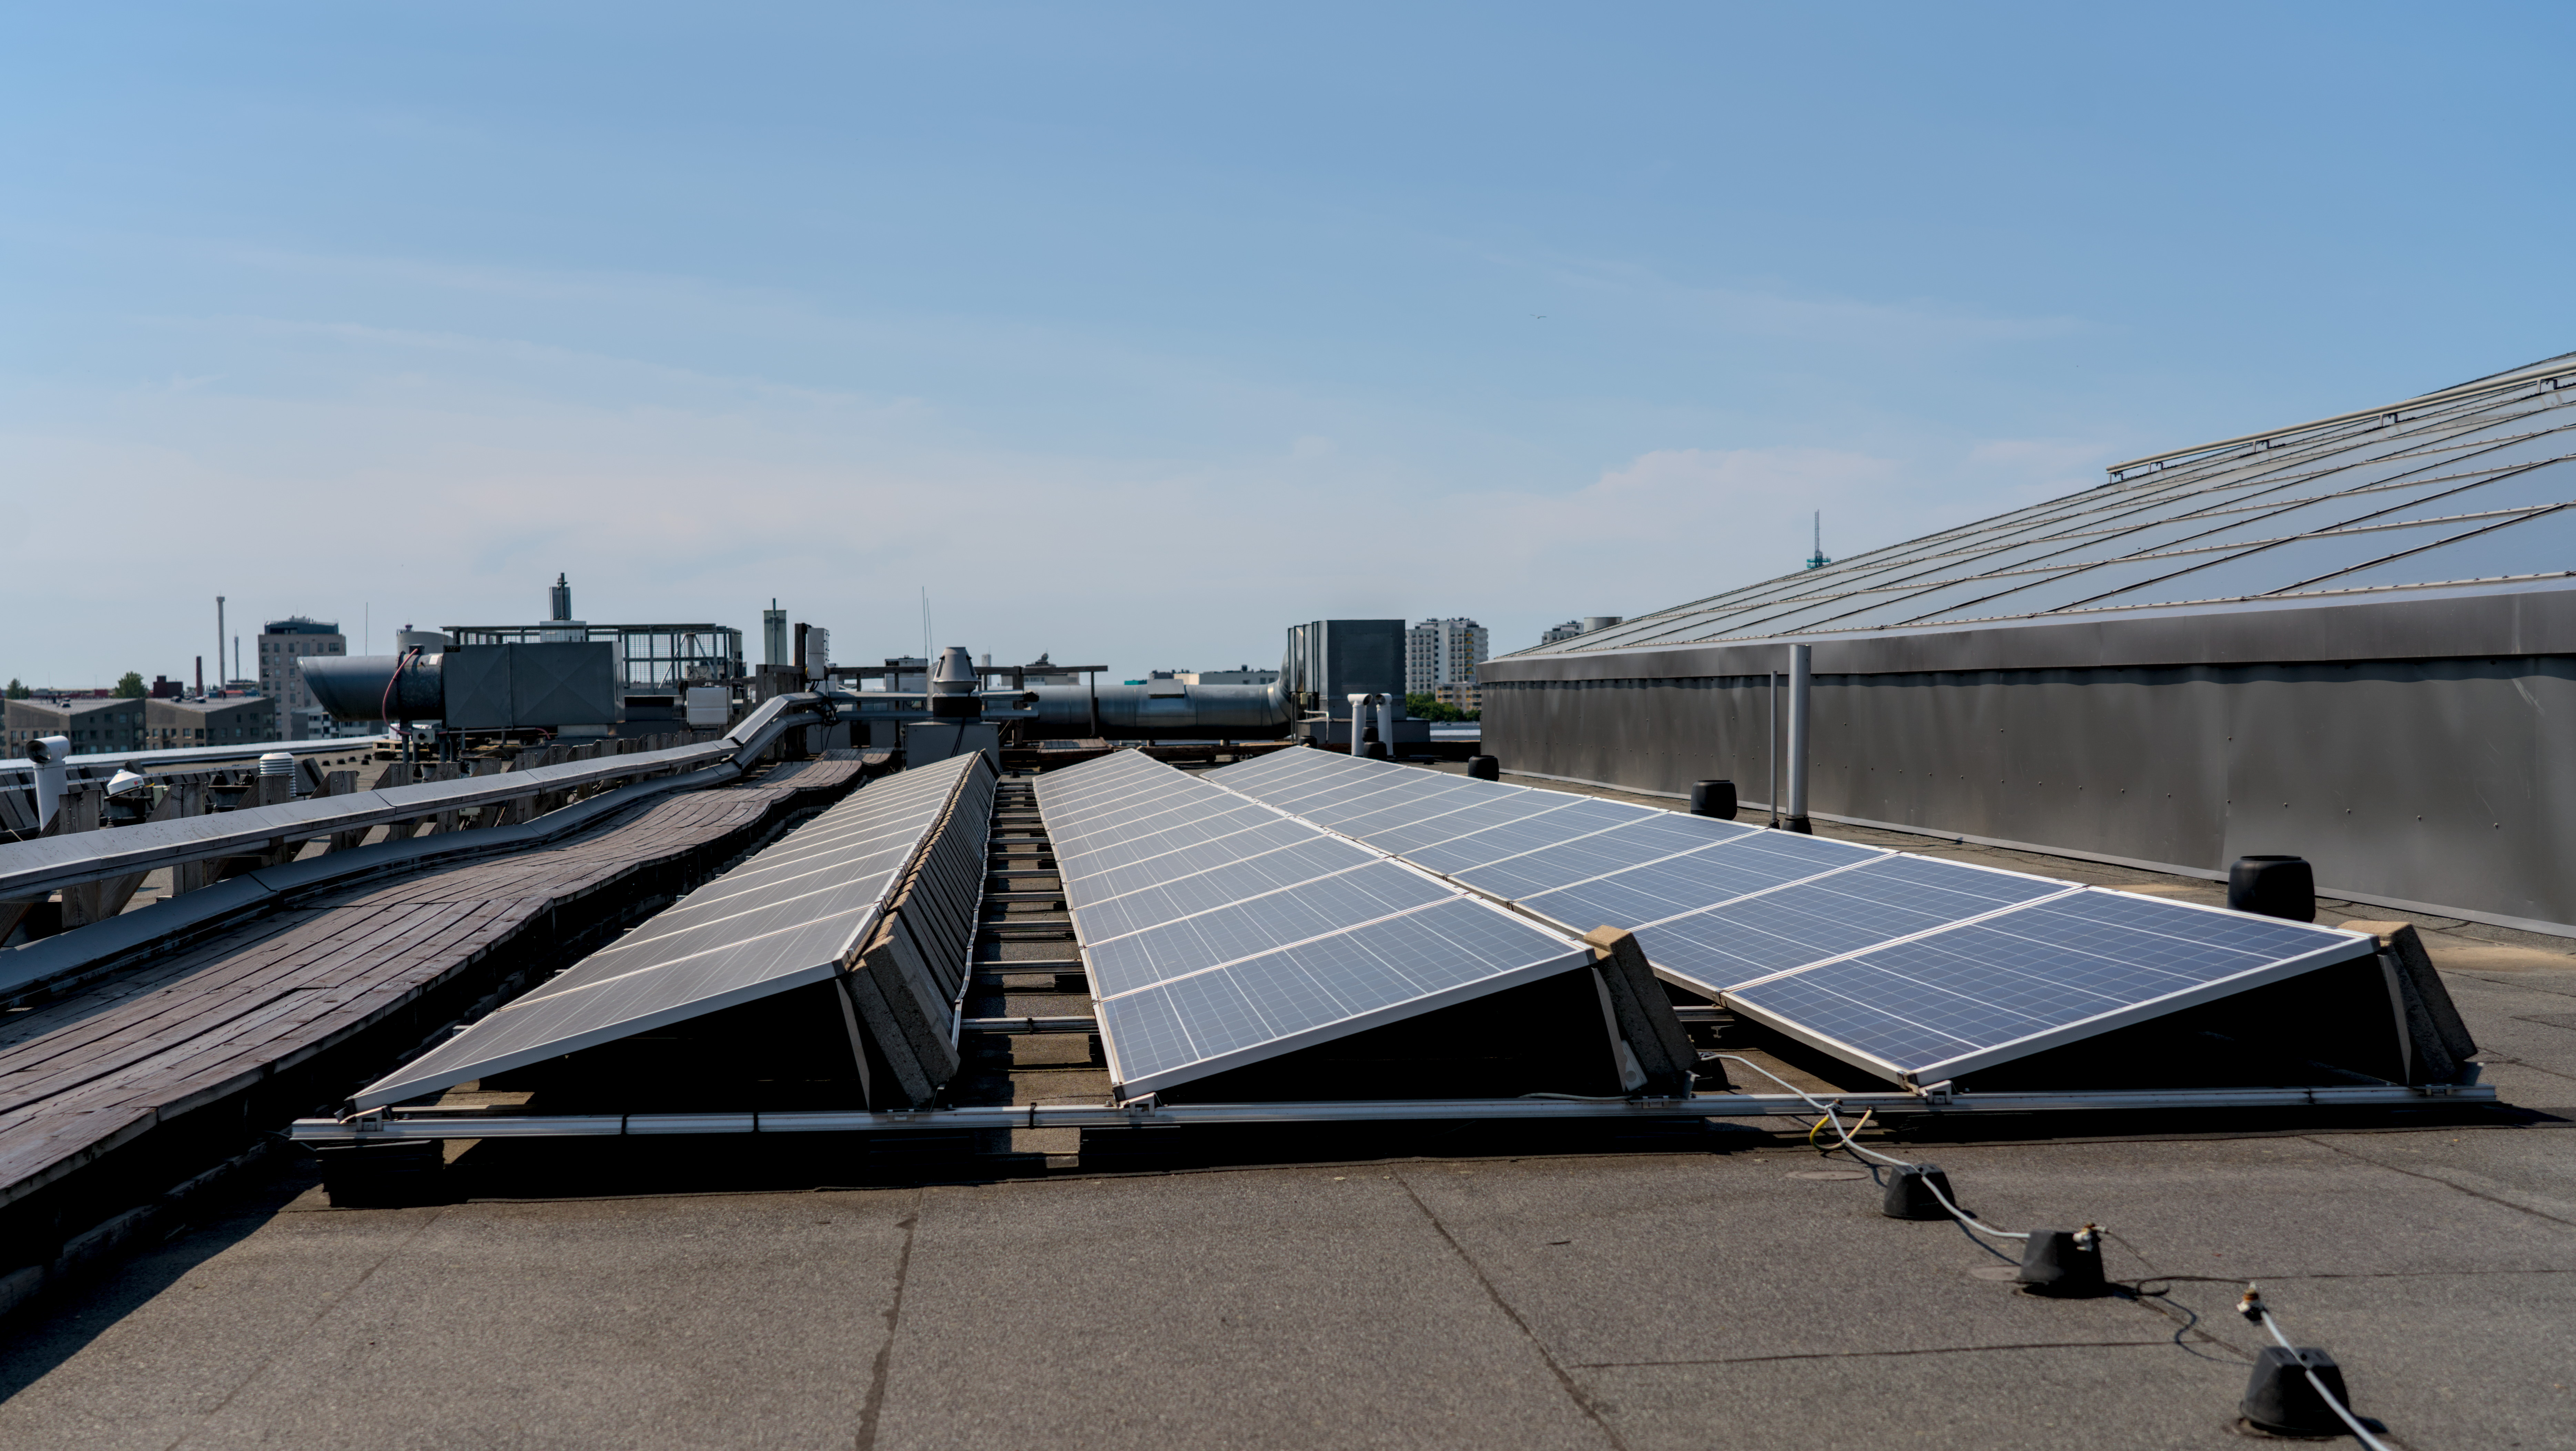
\includegraphics[width=0.9\linewidth]{pics/fmikumpula}
\figcaption{FMI Kumpula solar power installation string.}
\label{fig_fmikumpula_panels}
\end{figure}

%Both installations are installed on rooftops and there are no major obstacles causing shadowing for either installation. Smaller obstacles such as railings and instruments installed on the rooftop do however cast shadows on the PV panels with both Helsinki and Kuopio installations at low Sun angles. The same data was previously used in Herman Böök's \textit{Photovoltaic output modeling}\cite{hbook1} and thus installation parameters and datasets have previously been verified.

%The data in the two datasets follows the structure seen in Table \ref{table_fmi_kumpula_csv}. This snapshot from the Helsinki dataset shows that the temporal resolution is one measurement per minute and that there are four power values for each minute. Power values in columns String 1 and String 2 represent power output from two identical sets of solar PV panels, one of which is shown in Figure \ref{fig_fmikumpula_panels}. Electricity generated by these sets of solar panels is fed into the inverter and thus the inverter input should match the sum of String 1 and String 2. The inverter then converts the DC current from the PV panels to AC of a matching voltage to the buildings electrical system. Losses in the process should result in an inverter output value which is lower than the inverter input, but this does not appear to be true for every dataframe row. A plausible cause is the input/output measuring method which may result in noise in either input or output sides of the inverter.


%Datasets from other sources may have different temporal resolutions, units, or measuring points. From the consumer point of view, the inverter output is the useful power value and so this will be the power value used by algorithms in this thesis. Temporal resolution of the FMI data will be used as is.



\begin{table}[h]

\centering

\begin{tabular}{r|cccc} \hline\hline

Timestamp[UTC] & Inverter out & Inverter in & String 1 & String 2\\ \hline
$2015-08-26$ $03:34$ & $NaN$ & $NaN$ & $0.5$ & $NaN$\\
$2015-08-26$ $03:36$ & $11.1$ & $7.5$ & $2.6$ & $4.9$\\
$2015-08-26$ $03:37$ & $25.4$ & $26.1$ & $9.8$ & $16.3$\\
$2015-08-26$ $03:38$ & $30.7$& $NaN$ & $NaN$ & $0.4$\\
$2015-08-26$ $03:39$ & $46.4$& $44.8$ & $20$ & $24.8$\\
$2015-08-26$ $03:40$ & $3.3$ & $NaN$ & $NaN$ & $0.4$\\
$2015-08-26$ $03:41$ & $29.3$ &  $18$ & $9.1$ & $8.9$\\
$2015-08-26$ $03:42$ & $33.1$& $27.4$ & $10.6$ & $16.9$\\

\vdots & \vdots & \vdots & \vdots & \vdots\\
$2015-08-26$ $12:42$ & $12374.8$ & $14619.1$ & $7152$ & $7467.1$\\
$2015-08-26$ $12:43$ & $15442.2$ & $15482.1 $& $7708.9$ & $7773.2$\\
$2015-08-26$ $12:44$ & $14085.8$ & $12898.7$ & $6387$ & $6511.8$ \\
\vdots & \vdots & \vdots & \vdots & \vdots\\

\hline\hline
\end{tabular}

\tabcaption{A section from FMI's Kumpula solar site PV production data, only the timestamp and inverter output values are used by the algorithms in this thesis. All power measurements are in watts.}
\label{table_fmi_kumpula_csv}
\end{table}




%The figure \ref{fig_simplediagram} shows a simplification of how solar radiation radiation reaches the PV panel surface. 


%\begin{figure}[h]
%\centering
%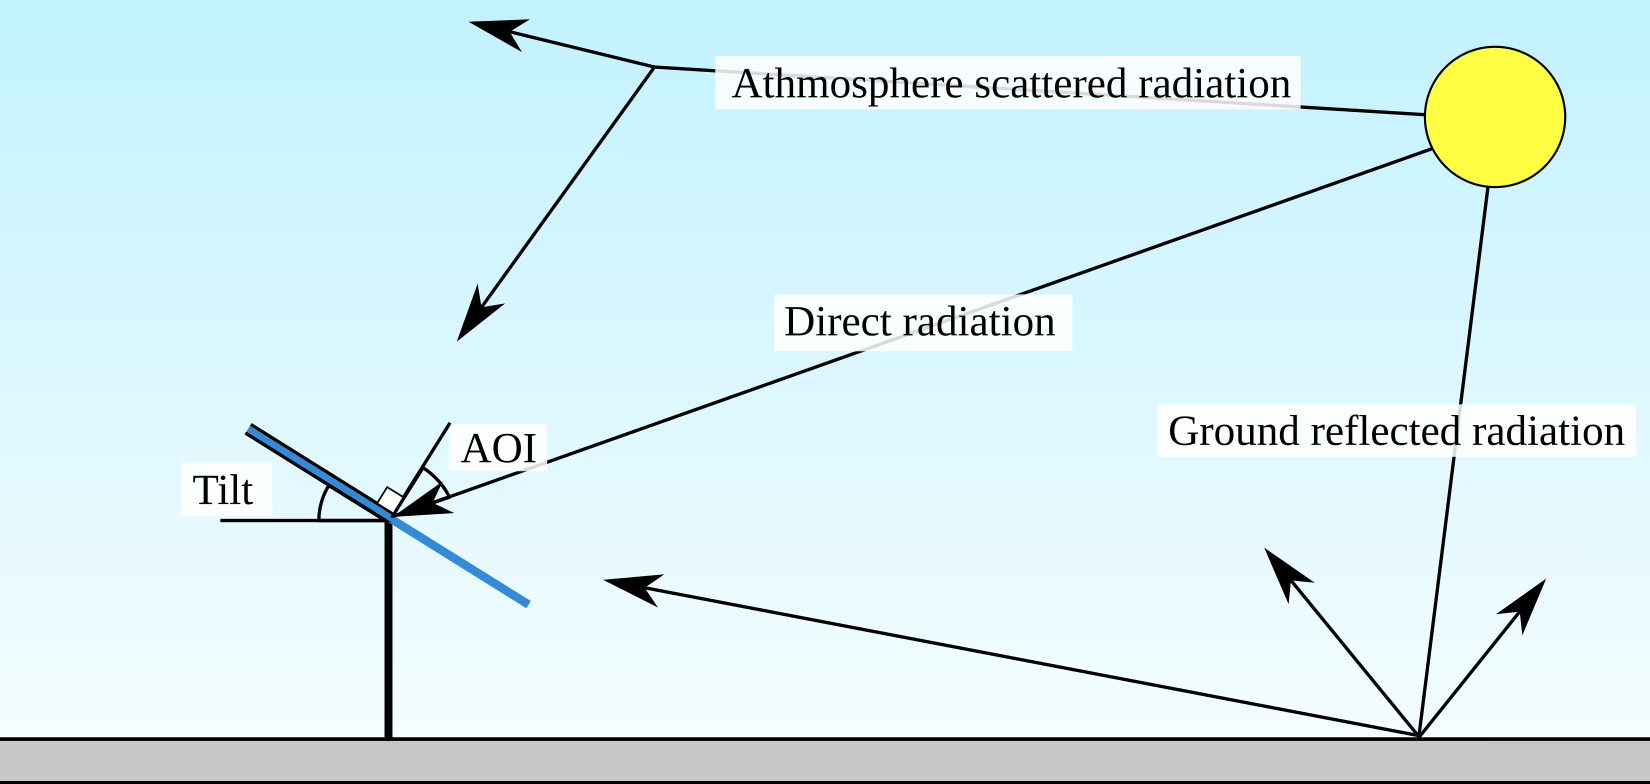
\includegraphics[width=0.8\linewidth]{pics/pvmodel2}
%\figcaption{Simplified installation diagram for a PV system in ideal conditions.}
%\label{fig_simplediagram}
%\end{figure}





%\section{Modeling PV panel as a surface}

%\noindent In the most basic PV model a 1m$^2$ solar panel can be approximated as a surface with a tilt and azimuth angles. Tilt and azimuth angles are used to describe the point of sky towards which the solar panel is oriented towards. Azimuth for north is 0 degrees and the rotation happens clockwise, tilt for a flat against the ground panel would be 0 degrees where as tilt of a wall mounted vertical panel is 0 degrees. The parameters given for FMI Helsinki and Kuopio installations in table \ref{table_fmi_helsinki_kuopio_parameters} tell us that the panels are nearly parallel to the roof where they are mounted on and that the Helsinki installation is oriented towards southeast and Kuopio towards southwest.

\begin{table}[H]
\centering
\begin{tabular}{r|cc} \hline\hline

 & Helsinki & Kuopio\\ \hline
 Latitude & $60.204^\circ$ & $62.892^\circ$ \\
 Longitude & $24.961^\circ$  &  $27.634^\circ$\\
 Nominal capacity &21 kW & 20.28 kW \\
 Panel tilt & $15^\circ$ & $15^\circ$ \\
 Panel azimuth & $135^\circ$ & $217^\circ$ \\
 Elevation & 17m & 10m\\
\hline\hline
\end{tabular}
\tabcaption{Parameters for the FMI's Kumpula(Helsinki) and Kuopio PV installations as listed in Böök 2020 \cite{hbook1}.}
\label{table_fmi_helsinki_kuopio_parameters}
\end{table}

%\noindent The nominal capacity of a PV panel is the peak output expected in optimal conditions. For a PV system the capacity or power rating is likely given as the sum of the nominal capacities per panel in the system. The panel elevation tells us how high the panels are from ground. This can be useful for modeling wind speed in more complex PV models.





%Figure \ref{fig_simplediagram} illustrates that there are three sources from which solar panels receive radiation. Direct radiation is the most simple of these to model as the effective solar panel surface can be easily calculated when the angle of incidence (AOI) is known and the AOI can be calculated when the position of the Sun and the panel angles are known. Ground reflected and atmosphere scattered radiation are more complicated to model as the sources of both are large areas, requring either integration or models which may otherwise be difficult to derive.


\clearpage

\section{Simple solar PV model} \label{section_simple_pv_model}
Let us create a simple model for how a solar PV system functions. This helps in explaining which parameters of a PV system are relevant for later simulating the output of a PV system and where they are used.

If we assume the electronical components such as inverters, cables and the solar panels themselves to be operating at a constant efficiency independent of ambient temperature and other factors, the output of a PV system can be approximated to be $\eta * P$ where $\eta$ is the combined efficiency of the solar panels, inverter and other electronic components and P is the sum of radiation reatching the solar panel surface. In a cloud free scenario we can assume P to be a function of panel angles, installation size and the position of the Sun. Figure \ref{fig_simplediagram} shows a visualization of the tree radiation types, each of which contributes to PV production.

\begin{figure}[h]
\centering
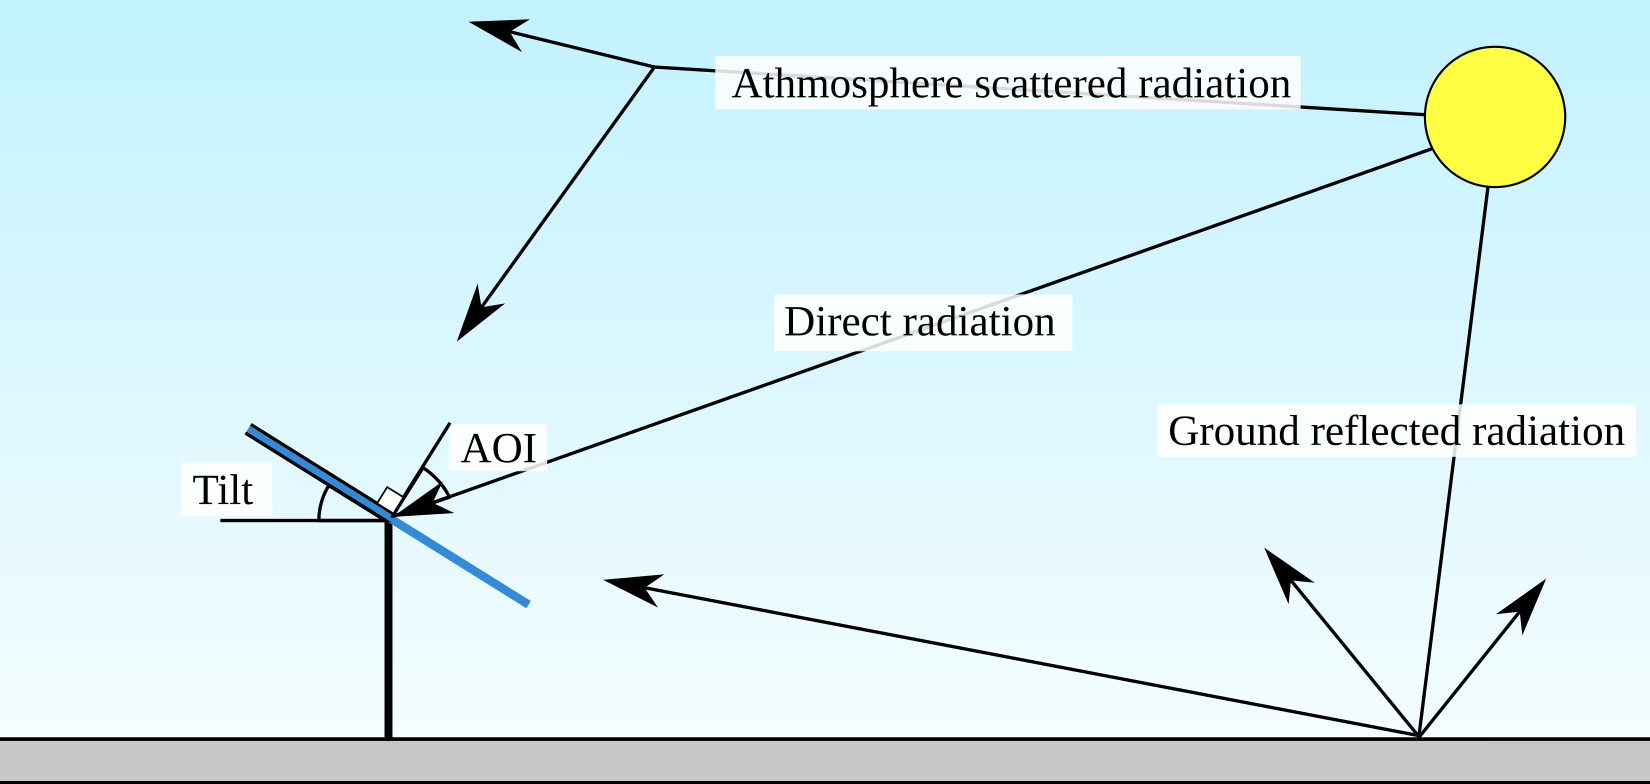
\includegraphics[width=0.8\linewidth]{pics/pvmodel2}
\figcaption{Simplified installation diagram for a PV system in ideal conditions.}
\label{fig_simplediagram}
\end{figure}

This figure contains a new angle AOI or the angle of incidence which has not been previously mentioned. AOI measures the angle between the solar panel normal vector and the incoming sunlight. As AOI approaches zero, from the perspective of direct radiation the relative surface area of the solar panel is at it's maximum resulting in higher amount of radiation per unit of surface area. And when AOI is 90$^\circ$ or greater, the panel surface does not receive direct sunlight. The observable position of the Sun which is required for calculating the AOI is a function of date, time and geographic location.

Note that this simple model does not take panel reflectivity or the loss of efficiency due to increased panel temperature into account and both of these topics will be discussed in later sections.



\section{Visualizing the data}
The Figure \ref{fig_oneyear_pointcloud} contains a 3D point cloud generated by plotting one year of data from the FMI Helsinki dataset, revealing visible structures in the data. The clearest structure in the 3D plot is the pattern formed by the first and last non-zero power minutes and this is later used for geolocation estimation. The second structure is the dome-like shape of the point cloud. This shape can be examined by taking one-day slices from the dataset and plotting them individually, as shown in Figure  \ref{fig_cloudfree_vs_cloudy}. These slices are used in later sections for panel installation angle estimation.

\begin{figure}[h]
\centering
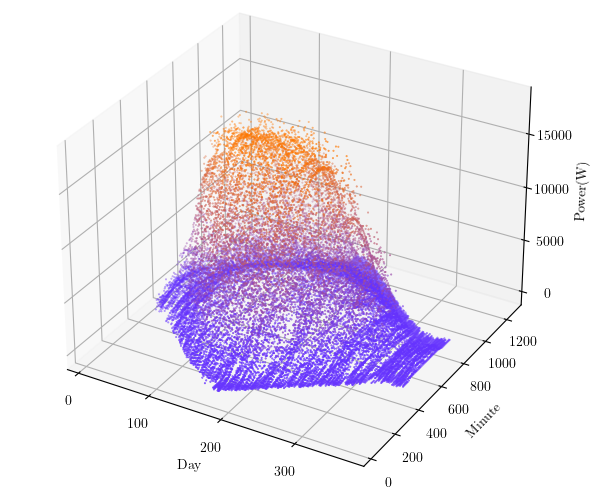
\includegraphics[width=0.8\linewidth]{pics/oneyear2}
\figcaption{One year of data from FMI Kumpula installation as a 3D point cloud.}
\label{fig_oneyear_pointcloud}
\end{figure}

\newpage
\begin{figure}[h!]
\centering
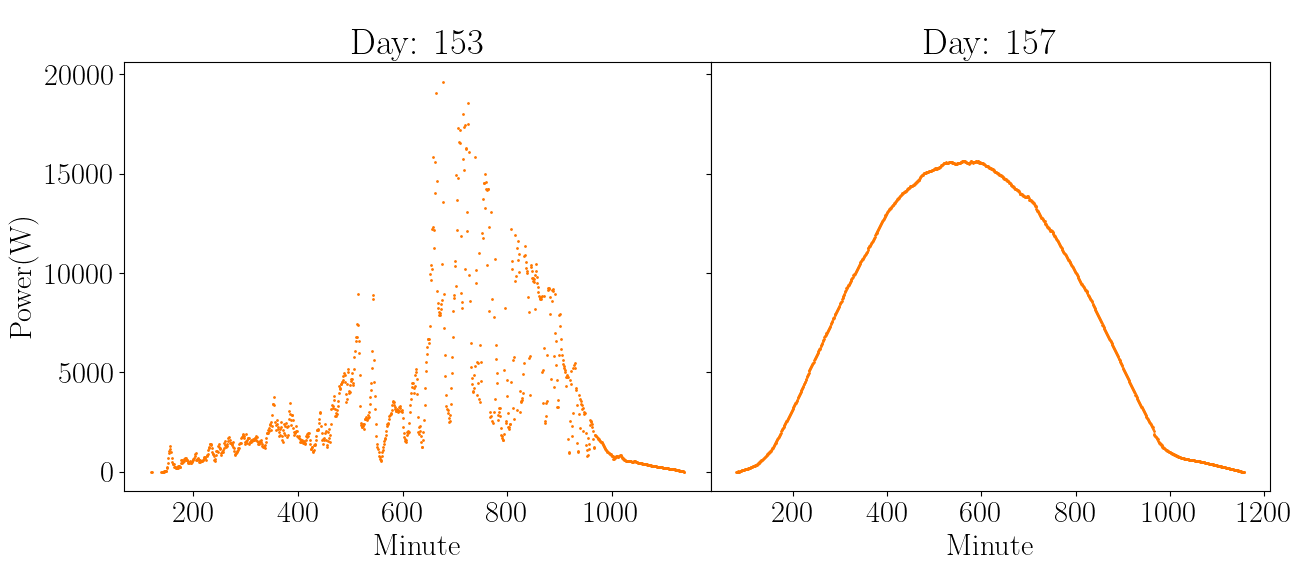
\includegraphics[width=1\linewidth]{pics/twodayshelsinki}
\figcaption{Two days from FMI Kumpula dataset with different charasteristics.}
\label{fig_cloudfree_vs_cloudy}
\end{figure}

\noindent The presumably cloud free day 157 in Figure \ref{fig_cloudfree_vs_cloudy} forms a skewed bell curve -like shape. This figure has a few notable features. The first and last non-zero minutes which occur somewhere around 100 and 1150 minutes can be useful for estimating the geographic location as they should correlate with sunsets and sunriseds. The peak of the plot at around 575 minutes may be a point in time during which AOI is rearching a daily mininmum. And finally the knee section beginning near 1000 minutes may represent a point in time where AOI reaches 90$^\circ$ and direct sunlight is no longer contributing to PV production.

For the cloudy day these same traits are much harder to measure. The first and last non-zero minutes appear to be nearly the same as suggested by earlier Figure \ref{fig_oneyear_pointcloud} but peak production minutes or transitions from indirect to direct sunlight are harder to clearly spot. The shape of the scatter plot is also irregular which may limit its usability. This would suggest that specific days may be preferable for analysis purposes.




\newpage
%\section{Data preprocessing}
%The data preprocessing required by the algorithms in this thesis can be split into two categories: classifying preprocessing and repairing preprocessing. Classifying preprocessing is used to determine if a certain section of data is suitable for analysis, the primary example here is the cloud free day detection algorithm which is discussed more throroughly in the next section. The second type of preprocessing, repairing preprocessing, involves using algorithms to fill gaps in the measurement data or otherwise attempt to repair data  which is unusable as is, but which could be used after repairing.

%The data preprocessing algorithms used in this thesis load the data from csv files and examine whether individual days in the dataset meet set qualification requirements. These are the minimum and maximum measurement count, whether first and last measurements are taken too close to minute 0 or 1439 and the the percentage of measurements included between the first and last measurement. Figure \ref{fig_accepted_days} contains a comparison on which days in the datasets met the requirements.


%\begin{figure}[h]
%     \centering
%     \begin{subfigure}[b]{0.48\textwidth}
%         \centering
%         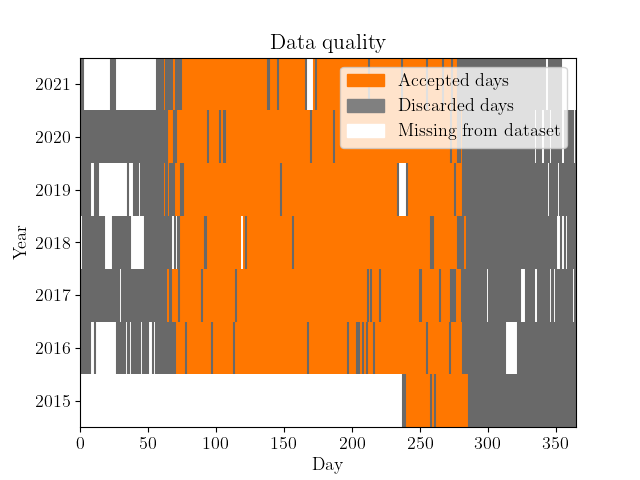
\includegraphics[width=\textwidth]{pics/helsinki_accepted_days}
%         \caption{Days in Helsinki dataset which met data quality thresholds.}
%         \label{fig_helsinki_accepted}
%     \end{subfigure}
%     \hfill
%     \begin{subfigure}[b]{0.48\textwidth}
%         \centering
%         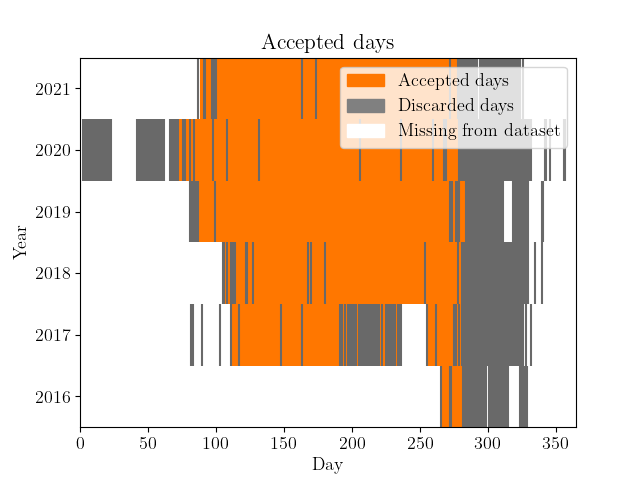
\includegraphics[width=\textwidth]{pics/kuopio_accepted_days}
%         \caption{Days in Kuopio dataset which met data quality thresholds.}
         
%         \label{fig_kuopio_accepted}
%     \end{subfigure}
%     \hfill
%     \caption{Requirements were measurement count between 400 and 1200, first minute is 5th or later, last minute is 1435 or earlier. More than 95\% of measurements between first and last minute must be included.}
%     \label{fig_accepted_days}
     
%\end{figure}


%\noindent After classification has discarded days that did not meet the set requirements, the next step is data repairing. The accepted days still contain a small amount of missing measurements and NaN values which can be linearly interpolated. This means that if a power measurement or a set of measurements is missing between two known datapoints, the missing values are estimated by a linear transition bridging the gap between the known datapoints. When noise is low, linearly approximating the missing values is unlikely to result in signficant errors. After this is done, the resulting data is ready for analysis.



\section{Clear day detection algorithm}
\label{clearskyalgo_chapter}
The ability to select days with clean power output data can be helpful for analysis purposes. The amplitude noise present in earlier Figure \ref{fig_cloudfree_vs_cloudy} would indicate that algorithmic cloud free day finding could be done by measuring how much sequential power measurements deviate from oneanother on average. The following listing describes one such algorithm.

%While previous preprocessing steps have filtered and repaired days according to measurement counts and data gaps, these algorithms did not filter days based on the amplitude noise present in power measurements. This power noise is typically induced by clouds, making the resulting power generation curves unreliable for curve fitting. The following algorithm can be used to automate the process of selecting days with minimal high-frequency fluctuations.


% If the interference in measurements caused by clouds or other sources is significant, the value of a day for model fitting is reduced. An example of strong interference can be seen in figure \ref{fig_cloudfree_vs_cloudy}. Detecting the presence of such interference with an algorithm would help with automating the process of model fitting as that would eliminate the need to manually select good days from datasets. The following steps describe the process used for cloud free day detection in this thesis.



%\noindent \textbf{Algorithm step by step:}

\begin{enumerate}
  \item Split dataset into individual days based on timestamps.
  
  \item Create a copy of the power measurements for each day and process this copy with a low pass filter algorithm.

  
  \item Calculate the difference between the original power values and the filtered power values. This delta value increases when high-frequency noise is present.
  
  
  \item Discard days with a delta value higher than a set threshold.
  

\end{enumerate}



\noindent The mathematically non-trivial parts here are threshold selection, difference measurement and low-pass filtering. Low-pass filtering is a term borrowed from the field of signal processing, and it refers to any algorithm that removes frequencies higher than a given limit from a signal, allowing lower frequencies to pass. 



Here the filtering is done with discrete Fourier transformations (DFT) and inverse discrete Fourier transformations (IDFT). When a list of numbers is used as the input of DFT, the output is a list of ordered complex numbers, each of which represents a sine wave of a certain frequency, phase and amplitude. The sum of these wave equations forms a continuous approximation of the input values and by sampling the continuous representation, the continuous trigonometric approximation can be transformed back into discrete values. However if the complex numbers are adjusted before the IDFT operation, frequencies can be selectively modified. This means that DFT and IDFT can be used for frequency specific modification of numerical lists, low-pass filtering being one of the possibilities. In this case the low-pass filtering was accomplished by zeroing out complex numbers which do not correspond to the 6 longest frequencies, the resulting smoothening can be seen in Figure \ref{fig_cloudfree_algo}.


While this process is somewhat complicated, Fourier transformations are not the only tool for creating low pass filters. Similar results can also be achieved by locally averaging each power value to be the average of nearest $k$ values. Discrete Fourier transformation based methods do however have an advantage in their universality. If the 6 or 7 or $n$ longest frequencies can be determined to be a good low-pass filter for PV power measurements, then these same frequencies should result in similar outputs no matter the temporal resolution of the power measurement data. Whereas a method based on local averages would require a different window size depending on measurement intervals.

The second component is not as complicated as the low pass filtering operation. Measuring the delta between a filtered and unfiltered set of measurements can be done by computing the discrete curve length or as was done here, measuring the absolute average deviation between filtered and unfiltered power measurement as per Equations \ref{eq2-1}-\ref{eq2-5}.


\begin{align}
Power &= [p_0, p_1, p_2, \dots , p_n]   \label{eq2-1}\\ 
Power_{filtered} &= [f_0, f_1, f_2, \dots , f_n] \\
Power_{delta} &= [|p_0 - f_0|, |p_1-f_1|, |p_2-f_2|, \dots , |p_n-f_n|] \\
delta_{avg} &= avg(Power_{delta}) \\
delta_{norm} &= delta_{avg}/ max(Power) \label{eq2-5}
\end{align}


\noindent The final component is threshold selection. The intermittent value $delta_{avg}$ describes the average wattage difference between measured and low pass filtered measured power values. By definition, this delta value is dependent on noise and installation size, limiting its usability. A noise only -delta value can be calculated by normalizing the delta with the $max(Power)$. The resulting $delta_{norm}$ should now be comparable between installations of different sizes. Choosing to reject every day for which $delta_{norm}$ value is higher than 0.05 would eliminate days with higher than 5\% normalized noise.




\begin{figure}[h]
\centering
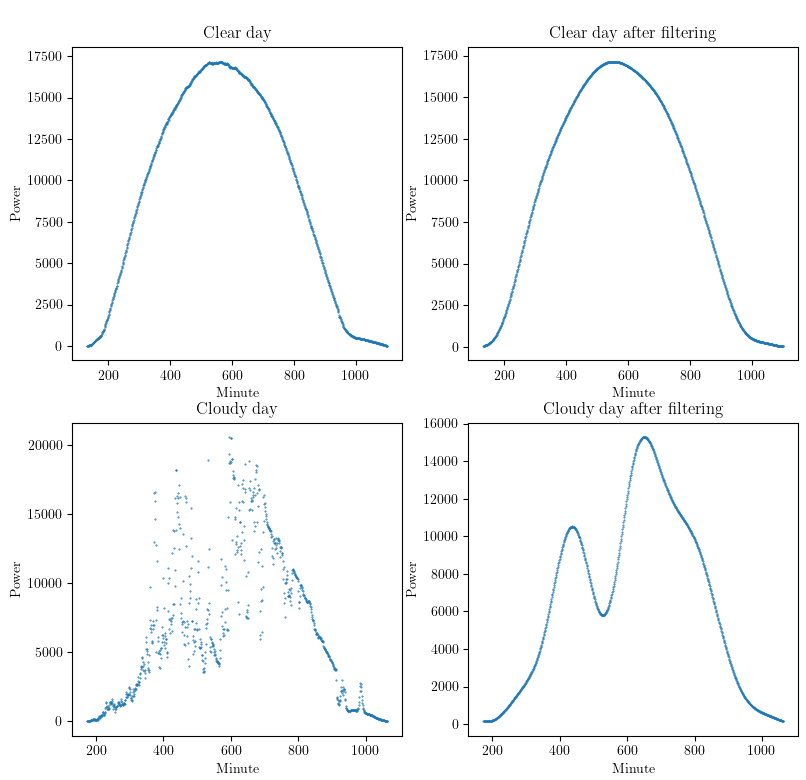
\includegraphics[width=0.8\linewidth]{pics/cloudfree_algo}
\figcaption{Cloud free day finder low pass filtering phase.}
\label{fig_cloudfree_algo}
\end{figure}



\newpage






%\noindent \textbf{Note:} that the algorithm listed above is highly dependent on measurement intervals and further tuning could be needed when operating with datasets that have different temporal resolutions. And as is, the algorithm selects days based on their proportionally low high frequency component, thus in theory this algorithm should classify zero power output days as cloud free days. Despite this fault the algorithm seems to work well for the FMI datasets.% as long as the input are selected to contain days close or between the spring and fall equinoxes. 



%The implementation of the clear sky algorithm seems to work well as indicated by \ref{fig-multidaypoavsmeasurements} but there are a few weak points in the algorithm as well. For example if a constant power day is given as the input for the algorithm, the algorithm will classify it as clear sky day even if a constant power day is more likely to be the result of faulty measuring instruments or errors in data preprocessing than a real cloud free day. In addition, the algorithm is unlikely to work well if sections are either removed from the measurements or if there is significant shading affecting the power output of the installation.

%\subsection{Difference between solar days and UTC days}
%For solar power analysis the concept of solar days is fairly useful. Solar days and sun based time measurement systems tend to rely on the angle of the sun and three 


%The timestamps used in solar PV measurements can be assumed to be in UTC +0 time. While this means that timezones or daylight saving time do not have to be accounted for, some operations may become more complicated as well since UTC days and solar days at do not always align. Note that here local solar day is defined as the 

%For example, if a one day slice is taken from a $0^\circ$ longitude installation power generation data, it is rather likely that the solar power generation would occur during an interval which centers around noon or 720 minutes. If the same slice is taken at $90^\circ$ longitude, this generation would be shifted by approximately 360 minutes. This is perfectly normal and expected behavior, but as a result, determining the first and last non-zero minutes of the day can be seen to nontrivial as per figure \ref{fig_poa0vs90}. In the $0^\circ$ plot, the first and last non-zero minutes are approximately 330 and 1100, but should the first and last minutes of the $90^\circ$ plot be defined as 0 and 750, 0 and 1420, -19 and 750 or something else entirely?


%\begin{figure}[h!]
%\centering
%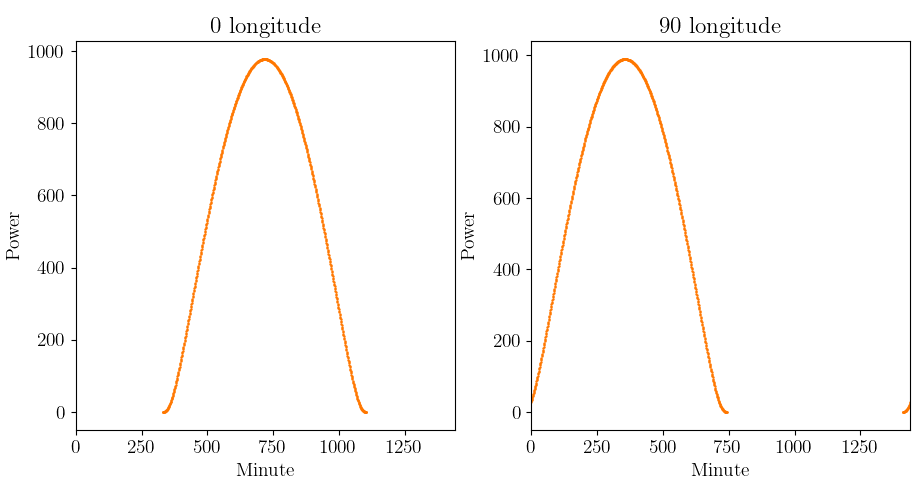
\includegraphics[width=0.9\linewidth]{pics/poa0vs90}
%\figcaption{Approximations of solar power generation at $0^\circ$ and $90^\circ$ longitude.}
%\label{fig_poa0vs90}
%\end{figure}


%\section{Third party datasets}
%Sunny portal etc here

%\section{Required assumptions}The algorithms presented in this thesis work on datasets which 


%Due to the diversity of possible solar PV installations, creating an universal model for parameter estimation is not fesiable. Installations could have been modified during operation, system failures could induce different types of changes in measurement data and 




%\section{Assumptions and possible issues}
%If metadata such as the geographic location or panel installation angles is missing from the datafiles, it is very likely that other critical pieces of information could be left out as well. Were additional modules were installed during operation? Could some panels be installed at different angles? What if the panels are installed in tracking mounts and thus the panel angles vary during each day? These questions are left unaswered and thus some assumptions have to be made. In this thesis we will assume that the panels are installed on fixed mounts, no changes were done during data gathering period and all panels are oriented similarly. We will also assume that there are no major obstacles casting shadows on the panels and that the panels are not self-shadowing, meaning that the panels are not casting shadows on one another.

%Another source of uncertainty is data collection itself. The device responsible for measuring power output values and logging the values has to have a clock for measuring time, but this clock could have be running too slow or fast, resulting in a drifting error in the timestamps. Similarly if the system clock is running at the right speed but it is off by a minute or two, this could cause a bias in the data which would be hard to detect. There is also the question of how measurement timing is done. If the time resolution of the logging device is 15 minutes, is the power value at 12:45 taken during the 45th minute or is the power value the average of the previous 15 minutes as is often done in meteorology? Or could the power value be the average of measurements taken during the interval 12:38 to 12:52? In meoteorology, the last period average would be the standard, but standards may not always be followed.

%is the standard, but standards are not always followed and thus 

%If enough time and effort was spent on algorithm design, in theory it could be possible to detect modifications to PV systems, the presence of variable panel angle systems and clock drifts. But these topics are outside the scope of this thesis and thus the assumption will be made that the 






















\chapter{PV output simulation}
The earlier PV model presented in section \ref{section_simple_pv_model} assumes PV output to be $\eta * P$. The value of $\eta$ can be difficult to accurately approximate due to differences in PV panel technologies, inverter efficiencies and other factors, but values in the range of 0.15 to 0.20 can be used as placeholders if a value is required. However for model fitting purposes $\eta$ does not need to be known as the if the shape of the curve is correct, the amplitudes of the curves can be matched.

The value $P$ has to be estimated. Physically accurate models are fairly complicated but luckily there are pre-existing tools made for solar PV modeling. The python library PVlib contains functions for estimating solar angles and different radiation types, the most relevant as of now being the POA irradiance. This plane of array irradiance is the sum of radiation reaching a $1m^2$ sized plane in clear sky conditions with given location, angles and datetime. A section of PVlib generated POA values are shown in Table \ref{table_poa_simulated_format}.





% accept that the model presented in earlier section \ref{section_simple_pv_model} is valid and 


%The primary tool used in this thesis for simulating PV generation with different parameters is the python library PVlib. PVlib contains be built functions for estimating solar irradiance, angle of incidence and a multitude of other useful tools. As seen in Table \ref{table_poa_simulated_format}, the plane of array(POA) simulations which estimate the irradiance per 1m² of solar panel surface resemble the earlier FMI PV datasets in their structure.

%An example of the irradiance simulation outputs is shown in table \ref{table_poa_simulated_format} and the table shows that the output format is simular to the FMI PV datasets shown earlier in table \ref{table_fmi_kumpula_csv}.




%Having a mathematical model which would simulate the output of a PV system would allow for the parameters of a PV installation to be solved with model fitting. In the best case scenario, we would have a physics based model which would take geographic location, panel installation angles, time of year and panel surface area or power rating as inputs and the output would be similar to the data from FMI Kumpula installation seen in table \ref{table_fmi_kumpula_csv}. Creating a such model is rather challenging as the model has to take into account atmospheric scattering, Sun angles, Sun-Earth distance variation and a multitude of other factors, the consideration of which are far beyond this mathematics thesis. Luckily the modeling of the energy output of solar PV installations has uses for the cost-benefit analysis of solar PV installations and thus pre-existing modeling algorithms are publicly available. 


% TODO REWRITE

%This thesis uses a plane of array irradiance simulation function from the python library PVlib. The function takes geographic location, timestamp and panel angles as inputs. The outputs contain power values which describe the amount of direct and atmospherically scattered light that would hit a square meter sized imaginary solar panel with the input parameters. The sum of these sources is referred as plane of array (POA) irradiance and this value can be used to estimate the output of solar power installations. A section of simulated data is included in table \ref{table_poa_simulated_format}.

%As the model simulates radiation values during clear sky conditions and not the power output of pv installations, the model should be seen as an approximation which is accurate to a certain degree. The differences between the model and recorded measurements could be due to reflectivity of the solar panels, weather conditions, temperature related changes in efficiency, atmospheric composition or a multitude of other factors which the model does not take into account.

\begin{table}[h]

\centering

\begin{tabular}{r|cccc} \hline\hline

Timestamp[UTC] & Minute & POA(W/m) \\ \hline
$2018-05-30$ $00:00$ &  $0$ & $0.0$\\
$2018-05-30$ $00:01$ &  $1$ & $0.0$\\
$2018-05-30$ $00:02$ &  $2$ & $0.0$\\
\vdots & \vdots & \vdots \\
$2018-05-30$ $ 07:34$ & $454$ & $800.691861$\\
$2018-05-30 $ $07:35$ & $455$ & $802.110516$\\
$2018-05-30 $ $07:36$ & $456$ & $803.517424$\\
\vdots & \vdots & \vdots \\
$2018-05-30$ $ 23:57$ & $1437$ & $0.0$\\
$2018-05-30 $ $23:58$ & $1438$ & $0.0$\\
$2018-05-30 $ $23:59$ & $1439$ & $0.0$\\

\hline\hline
\end{tabular}
\tabcaption{One day of simulated clear sky plane of array irradiance values. Note that the minute column is added to the table for convinience and it is reduntant as minutes can be read from the timestamps.}
\label{table_poa_simulated_format}
\end{table}


%\subsection{PVlib POA function inputs} 
%PVlib plane of array irradiance can be simulated with 

%\begin{lstlisting}[caption={PVlib POA simulation function header.}, label={poa_header}]
%def get_irradiance(year, day, lattitude, longitude, tilt, azimuth):
%\end{lstlisting}


%\noindent The following listing contains the relevant parameters of the plane of array irradiance function and their domains.
%The POA simulation function accepts real --or integer as is the case with the day parameter-- valued parameters in the ranges listed below. 

%\begin{itemize}
%	\item Year $\in \mathbb{N}$
%	\item Day [1, 365/366] $\in \mathbb{N}$
%	\item Latitude [-90, 90] $\in \mathbb{R}$%, Finland fits within subrange [59, 70]
%	\item Longitude [-180, 180]  $\in \mathbb{R}$%, Finland fits within subrange [19, 32] 
%  	\item Tilt [0, 90] $\in \mathbb{R}$
%  	\item Azimuth [0, 360[ $\in \mathbb{R}$
%\end{itemize}

%\noindent \textbf{Note:} While the function does accept the full latitude and longitude ranges as inputs, it may be beneficial to restrict the range of the coordinate parameters when the approximate location of the installation is known. For example, Finland fits within subrange [19, 32] on the longitude axis and thus it could make sense to restrict the longitude range when examining installations located within Finland.
%
%\vspace{3mm}
%\noindent
%The day and year parameters can be assumed to be always known as datasets include timestamps and this leaves four unknown system parameters. These four parameters span a 4D parameter space of possible PV installations. The size of this parameter space is connected to the difficulty of the parameter estimation problem. As the parameters are in $\mathbb{R}$, the amount of sensible combinations is the product of the discretization of each of the parameter ranges. Tilt and azimuth parameters can be discretized as integers, resulting in $90*360$ or $32400$ unique angle space points. The geographic latitude and longitude coordinates are somewhat harder to discretize. In an arbitrary 0.1 degree geographic discretization there would be $1800*3600$ or 6480000 coordinate combinations. The product of these two sums results in $2*10^{11}$ unique parameter combinations.

%A parameter space this large is difficult to examine exhaustively. Even a system capable of evaluating 100 000 angle space points per second would need approximately 23 days in order to evaluate all of the possible combinations. However if the parameters can be solved in isolation from oneanother, the required computational time would decrease significantly. Instead of $90*360*1800*36000$, there would be $90+360+1800+3600$ combinations to evaluate. This highlights how important it is to break problems into smaller pieces whenever possible and much of this thesis focuses on how this can be done with solar PV parameter estimation. 


\newpage
\section{PVlib POA evaluation}
Before the PVlib POA simulations are used for parameter estimation, the simulated values should be compared with known PV measurements. Figure \ref{fig-multidaypoavsmeasurements} contains 6 days from FMI Kumpula dataset year 2017 plotted on orange and PVlib simulated POA values with the parameters of the Kumpula installation. Power values of the POA simulations were multiplied by 19 in order to match the magnitudes of both plots.

This plot shows that in presumably cloud free conditions during days 123, 136 and 141 the POA values and real PV output curves have matching shapes with minor deviations. And during days 70, 150 and 240 clouds, snow or other factors have caused noise into power generation resulting in deviation between the measurements and the PVlib POA simulation. This noise appears to result in both increases and decreases in expected power generation. Decreases are fairly intuitive as clouds can block direct solar radiation from reaching panel surfaces but positive noise can be unintuitive and it has implications for model fitting. Well positioned clouds can reflect additional sunlight onto the panels or snow near panels may increase ground reflectivity. This noise charasteristic means that local maximums or minimums of power measurements can not be used to approximate the expected power output in normal conditions. 




%Before implementing the parameter estimation functions, the POA simulations should be tested against known measurement data. Figure \ref{fig-multidaypoavsmeasurements} displays that in clear sky conditions the pvlib irradiance model is following real world measurements closely with a few exceptions. And during cloudy days the measurements are often lower than the clear sky model would indicate, but they can also peak higher than they would during cloud free days. These increases of power generation above clear sky estimated power are likely to be caused by the additional sunlight reflected from clouds towards solar panels in partly cloudy weather conditions and it shows that cloud induced noise can be positive as well as negative. 


% Power output of FMI Kumpula PV installation and the pvlib POA simulation computed with the parameters from Table  \ref{table_fmi_helsinki_kuopio_parameters}. Horizontal axis on the graphs corresponds to time and vertical axis marks the estimated power values. The purpose of the graphs is to display the different shapes and deviations from POA models and thus axis names and numbers were left out. Upper row contains randomly selected days while as the lower row has days chosen by a clear sky algorithm mentioned in Chapter \ref{clearskyalgo_chapter}. Measurements are from 2017. POA irradiance values were multiplied by 19 in order to match the curves values on power axis.
\begin{figure}[h]
\centering
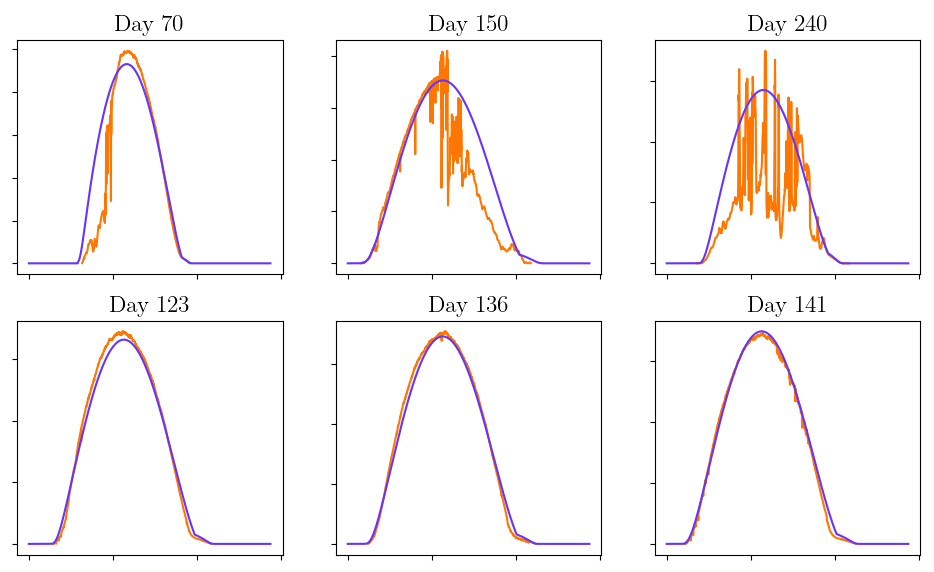
\includegraphics[width=0.9\linewidth]{pics/multiday_vs_neat}
\figcaption{Plots comparing POA simulations with real PV measurements from FMI Kumpula dataset year 2017.}
\label{fig-multidaypoavsmeasurements}
\end{figure}



% On the 70th and 150th day, the first and last minutes do not seem to be exactly the same as in the simulation, but the difference seems minor and it is occuring in different directions.






%\textit{The following claims are unverified conjectures, but the smooth shape and the early date of the first graph could hint that the increased peak production on the 70th day could be due to reflections from snow, while as the more irregular production on the 150th and 240th day would seem to indicate that the variation is caused by clouds. Filtering out days such as the 150th or the 240th from the dataset should be rather simple as the high frequency component is noticeable, but low frequency deviations such as the smooth increase in production of the 70th day could prove to be more difficult to detect algorithmicly.}






\newpage
%\section{Influence of different parameters on the PVlib poa model}
%\label{influence_parameters}



\begin{figure}[ht!]
\centering
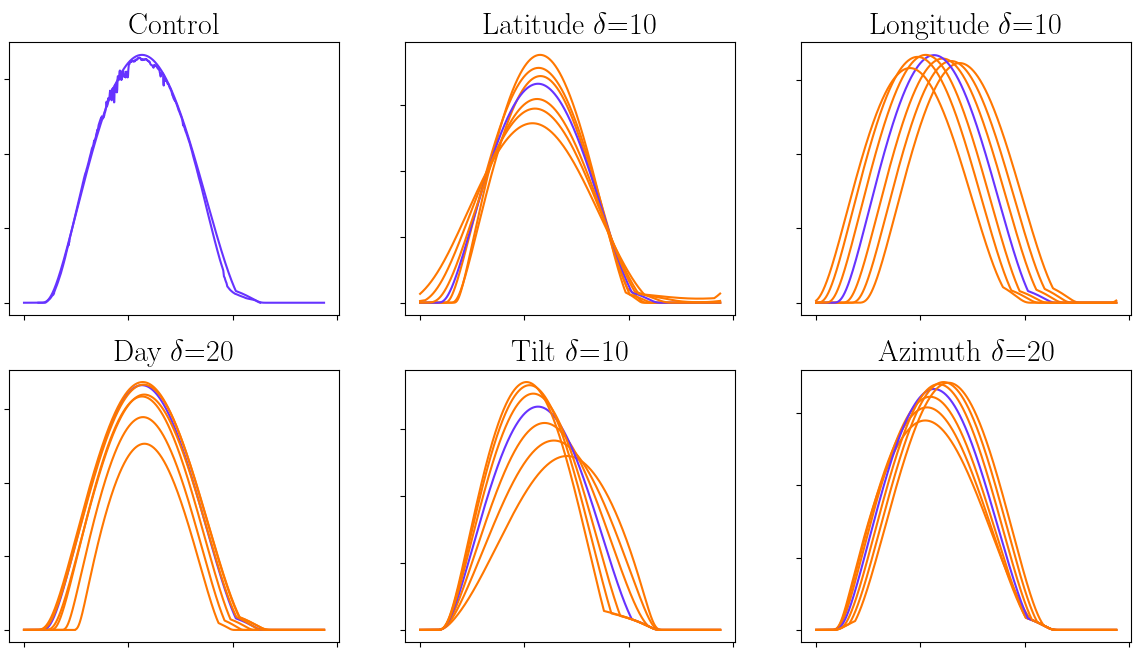
\includegraphics[width=0.9\linewidth]{pics/poa_eval_new_crop}
\figcaption{Influence of changes in PVlib simulation parameters on generated power output curves. Control shows FMI Helsinki measurements and simulation with the same parameters as the Helsinki installation. Simulated power values are multiplied by 19 in order to match values on y-axis.}
\label{fig_poa_different_parameters}
\end{figure}

\noindent By varying the different simulation parameters as shown in Figure \ref{fig_poa_different_parameters}, we can examine the relationships between parameters and power generation curves. This can help us understand if there are usable patterns in the data. In the best case scenario each of the simulation function inputs would affect one measureable property in the irradiance plots and their relationship would be bijective. To give an example, if the peak power minute was isolated from all other parameters than the longitude and the relationship between longitude and peak power minute was linear, it would be possible to solve the peak power minute to longitude function with just a few plane of array irradiance simulations.

In the exact opposite case where every measureable property of irradiance plots is affected by every input parameter, solving the parameters would be much harder or even impossible. For example if all of the parameters influenced the same traits to different extents and the system was not bijective, multiple parameter combinations could result in the same simulated power graph. In a such system there would not be a single solution but rather a set of possible solutions.

\newpage The problem of solving installation parameters would appear to be somewhere in between the two extremes. The longitude parameter would seem to shift the curve along the time axis whereas tilt and azimuth parameters do not affect the first or last non-zero minutes but they do affect the shape of the curve. Observations of parameter to trait interactions are listed in Table \ref{table_traits}.



\begin{table}[H]
\centering
\begin{tabular}{r|cc} \hline\hline

 Parameter & Traits affected\\ \hline
 Latitude & Shape, first and last minute times\\
 Longitude & First and last minute times\\
 Tilt & Shape\\
 Azimuth & Shape\\

\hline\hline
\end{tabular}
\tabcaption{Function input to observed trait table.}
\label{table_traits}
\end{table}


%Base on these observations, the relationship between longitude and the First and last minute times would seem like the best starting point for parameter solving.

%If the POA model is assumed to be accurate, the model could be used to simulate the effects of different parameters on power generation. This could provide insights into the relationship between patterns in the data and the parameters of the system. The relevant parameters to simulate and their default values can be seen in table \ref{table_default_parameters_poa_simulations}. In the following simulations, only one of the default parameters is varied. This is done in order to isolate the effect of individual parameters.



%\begin{table}[!ht]
%\centering
%\begin{tabular}{r|c} \hline\hline

% Parameter & Value \\ \hline
% Day & $180$  \\
% Latitude & $60^\circ$  \\
% Longitude & $28^\circ$  \\
% Panel tilt & $30^\circ$ \\
% Panel angle & $180^\circ$  \\
%\hline\hline
%\end{tabular}
%\tabcaption{Default parameters for POA simulation used in this section. }
%\label{table_default_parameters_poa_simulations}
%\end{table}


\newpage

\subsection{Influence of different longitudes}
\label{section_different_longitudes}

\begin{figure}[ht!]
\centering
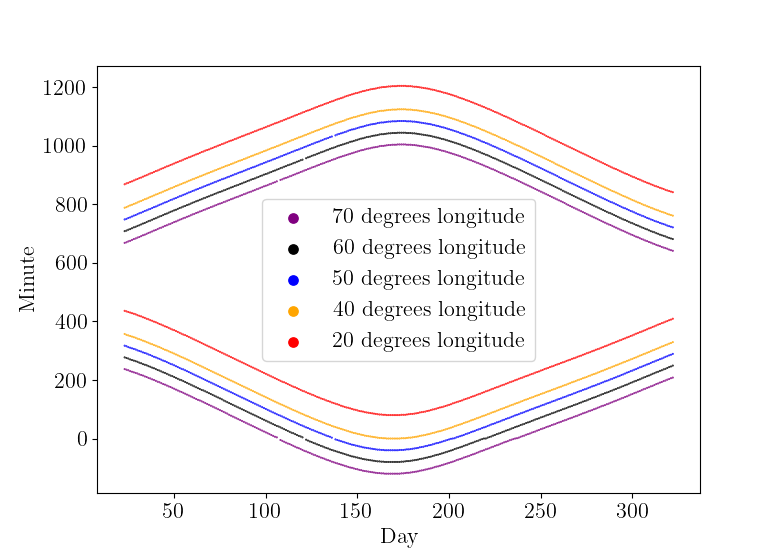
\includegraphics[width=1\linewidth]{pics/poa_var_lon}
\figcaption{First and last non-zero minutes of each day from year long simulations at different longitudes.}
\label{fig-poa_var_lon2}
\end{figure}

\noindent Based on earlier observations listed in Table \ref{table_traits}, solving the longitude of installations would seem like a sensible starting point. The figure comparing the effects of different parameters seemed to suggest that the relationship between longitude and significant minute times is very close to linear and the same is seen here in Figure \ref{fig-poa_var_lon2}. In Hagdadi 2017 \cite{navid_australian_article} and in Williams 2012 \cite{older_solar_solver_article} this relationship was used in order to determine the geographic longitude. The algorithms used by both of the articles relies on calculating an approximation for the time of the solar noon based on the average of the first and last minutes, this solar noon minute is then translated into a geographic longitude coordinate.





%There are at least two ways of estimating the longitude from the UTC solar noon time. First method is based on fitting a linear equation to a list of known solar noon to longitude-pairs. This would result in an equation of the form $f(x) = 0.25^\circ* x + b$ where the solar noon minute $x$ is multiplied by the constant $0.25$. The constant of $0.25^\circ$ comes from dividing a full circle by the amount of minutes in a day, 1440. The constant $b$ is around $-180^\circ$ and it is the result of solar noon occuring close to noon.
%In the figure \ref{fig-poa_var_lon2}, the relationship between the first and last minutes of a day and the geographic longitude can be seen to be linear. This linear equation should be of the form $f(x) = 0.25^\circ* x + b$ where the solar noon minute $x$ is multiplied by the constant $0.25$. The constant of$0.25^\circ$ comes from dividing a full circle by the amount of minutes in a day, 1440. The constant $b$ is roughly $-180$ degrees as that is the offset required for adjusting solar noon from



%and the figure \ref{fig-poa_var_lon2} it would seem that the relationship between longitudes and first and last minutes is a good starting point for parameter so


%at least very close to linear. In Hagdadi 2017 \cite{navid_australian_article} and in Williams 2012 \cite{older_solar_solver_article} this relationship was used in order to determine the geographic longitude. The algorithms used by both of the articles relies on calculating an approximation for the time of the solar noon based on the average of the first and last minutes, this solar noon minute is then translated into a geographic longitude coordinate.

% and a similar algorithm is detailed in []..




\newpage

\subsection{Influence of different latitudes}
\label{section_different_latitudes}

\begin{figure}[ht!]
\centering
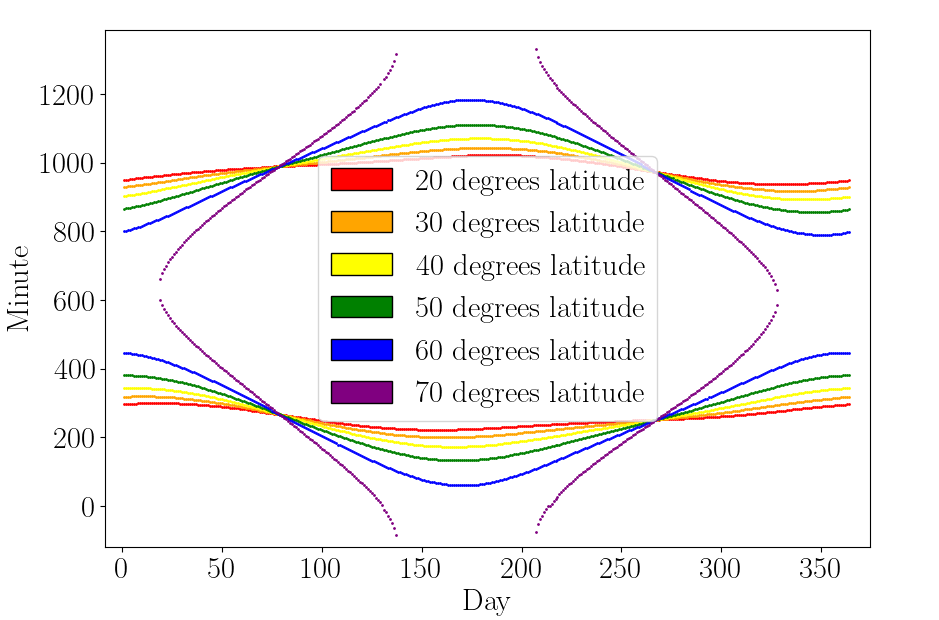
\includegraphics[width=1\linewidth]{pics/different_latitudes}
\figcaption{First and last non-zero power minutes of each day from year long POA simulations at different northern latitudes.}
\label{fig_poa_var_lat}
\end{figure}

\noindent The latitude simulations in Figure \ref{fig_poa_var_lat} show that the day length stays fairly consistent at lower latitudes but with latitudes of $50^\circ$N and higher, the day lenghth becomes significant. This variation in day lengths can be consistently measured near equinoxes as day lengths are always well defined.

%for locations close to the equator, but with latitudes of $50^\circ$ and higher, the day to day variation is significant. These POA simulations would imply that the region around equinoxes is ideal for day length based analysis as there day length is always well defined and the rate of change can be measured. 


\newpage

\section{Increasing the accuracy of solar PV simulations}
\label{section_increased_accuracy_simulations}


\begin{figure}[h]
\centering
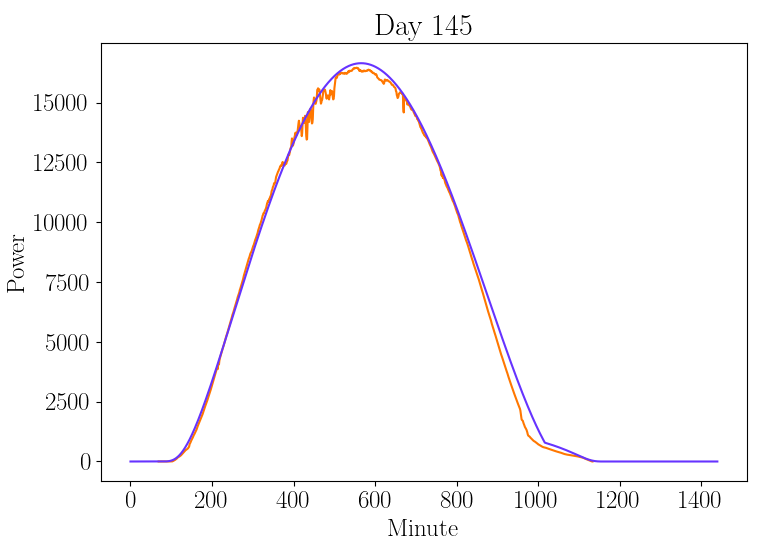
\includegraphics[width=0.7\linewidth]{pics/poa_eval_single_day}
\figcaption{Figure comparing Kumpula PV measurements on orange and PVlib simulated clear sky POA irradiance(purple). POA power values were scaled with a multiplier in order to match curve magnitudes.}
\label{fig-poa_eval_single_day}
\end{figure}

\noindent 
Figure \ref{fig-poa_eval_single_day} and the earlier multi-day comparison Figure \ref{fig-multidaypoavsmeasurements} both suggest that PVlib POA estimates are a fairly good approximation of clear sky PV output. However when examined more closely, there are some deviations between the POA simulations and real PV outputs. The PVlib simulations suggest a higher than achieved output near 580 and 1000 minutes. 

At 1000 minutes this is likely a result of reflective losses as the radiation reaching a panel surface is not equal to absorbed radiation and with south-east facing panels the direct component of solar radiation would be reaching the panel surfaces at shallow angle, increasing the fraction of radiation reflected away from the panel surface. This means that a more accurate PV model would have to take panel reflections into account in order to correct for this discrepancy between the model and the PV measurements.

Near 580 minutes the panels are absorbing a high amount of radiation. If we assume the solar panels to be operating at approximately 20\% efficiency, 80\% of incoming radiation is transformed into heat and the efficiency of PV panels and many other electrical devices is dependent on operating temperature. This would also explain the negative noise present during the peak output hours as gusts of wind may be enough to cool the panels enough to cause noise patterns in the PV data. This noise is difficult to estimate, but panel temperature modeling could be included in a better PV model and this may result in higher estimation accuracy near peak production times.



%Figure \ref{fig-poa_eval_single_day} compares the simulated and measured PV output during a sunny day in Helsinki. The shapes of the curves match quite closely, but there are some discrepancies. The estimated power values for the peak production hours are higher than measured power values and a similar phenomena is seen near minute 1000. These discrepancies can be explained by real world phenomena as PVlib POA values describe the amount of radiation reaching the surface of a solar panel. This is different from the power output of a PV system as thermal losses and panel reflections are not taken into account. This section examines an improved PV model which includes these losses.

\newpage

\subsection{Improved PV model}

\begin{figure}[h]
\centering
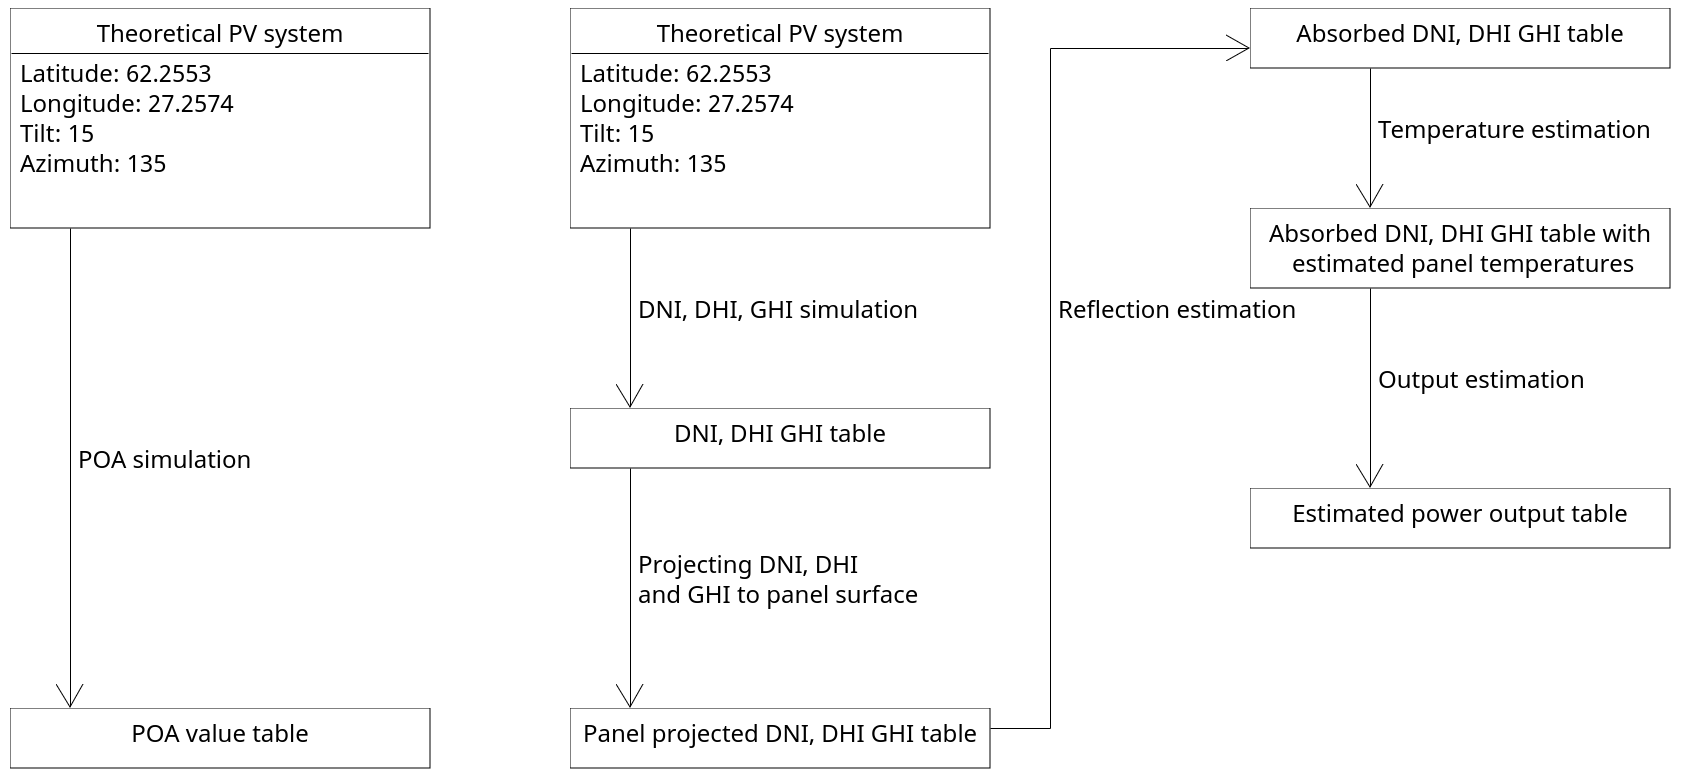
\includegraphics[width=1.0\linewidth]{pics/uml2}
%\captionsetup{labelformat=empty}
\figcaption{Original POA-based PV model and the improved model with reflection and temperature estimation.}
\label{fig-pv_model}
\end{figure}


\noindent 
Figure \ref{fig-pv_model} contains a comparison of steps required for PVlib POA based solar PV output estimation and the steps of a more physically accurate PV model. While the steps required by the methods may seem different, they are very similar.

When the PVlib POA model is used, PVlib internally calculates estimates for DNI, DHI and GHI, each of which is a component of solar irradiance, and then transposes the irradiances to the solar panel surface. The sum of the radiation types after transposition is the plane of array irradiance or POA. However if we use PVlib to generate a table of the three radiation components, we can then transpose the radiation types to the panel surface with our own models for transpositions, reflection estimation, panel temperatures and the output of the PV system. The three irradiance types were mentioned earlier as direct radiation, atmosphere scattered radiation and ground reflected radiation but in meteorology they go by the following names.



\begin{itemize}
\item DNI is direct normal irradiance which represents direct sunlight received by a 1m² -sized plane with AOI of 0 degrees. Note that DNI consists of only direct sunlight and atmospherically scattered light or ground relfections are not components of DNI.

\item DHI is diffuse horizontal irradiance which represents the irradiance reaching a shaded 1m² -sized plane with tilt of 0 degrees. DHI represents atmosphere scattered radiation and DHI can be measured with an instrument which blocks direct sunlight.

\item GHI is global horizontal irradiance and it represents the amount of irradiance per 1m² -sized plane with tilt of 0 degrees. GHI is made up of direct irradiance and atmosphere scattered irradiance. GHI combined with albedo can be used to estimate the ground reflected irradiance.
\end{itemize}

\noindent
%These irradiance types are present in both the simpler PVlib POA based model and the improved PV model. The difference between the two models is that in the POA-model, PVlib internally calculates three irradiance components DNI, DHI and GHI and projects them to the panel surface, returning the resulting sum as plane of array irradiance. Where as in the more complex PV model, PVlib estimates DNI, DHI and GHI, each of which are processed by multiple functions before they are combined into an estimated power output value, resulting in a physically more accurate PV output estimation.

\subsection{Panel surface transpositions}

The first step in the improved model is panel surface transposition. Sandia National Laboratories, the original author of PVlib, suggests the following two equations for DNI and GHI transposition and five alternative models for DHI transposition. Perez 1990 model \cite{perez} was chosen for DHI transposition due to the use of the model by a co-worker at FMI and inclusion in Sandia suggested projection models \cite{sandia_poa_dhi}. Chosen DNI and GHI transposition models are shown below. DHI Perez transposition model utilizes number tables and as a function included in PVlib was used, the mathematical notation for the method was left out. See thesis source code for the implementations.

%As there are three irradiance types with different apparent sources and thus directions, three irradiance projection functions are needed. The simplest way to project DNI and DHI to panel surface is to use the equations $DNI_{proj}= DNI* sin(AOI)$ and $DHI_{proj}= DHI* sin(tilt)$ both of which are mathematically trivial. However ground reflected irradiance projection is not as simple. The original author of PVlib, Sandia National Laboratories recommends the use the following two equations for DNI and GHI, offering five different models for DHI. 


\noindent\textbf{DNI transposition}\cite{sandia_poa_dni}
%
\begin{equation}
\begin{split}
\label{sandia_eq_dni}
DNI_{poa}(DNI, AOI)= DNI*cos(AOI)
\end{split}
\end{equation}
Where $AOI$ is the angle of incidence.


\noindent\textbf{GHI transposition}\cite{sandia_poa_ghi}
%
\begin{equation}
\begin{split}
\label{sandia_eq_ghi}
GHI_{poa}(GHI, albedo, tilt)= GHI*albedo*\frac{1-cos(tilt)}{2}
\end{split}
\end{equation}

\noindent Where 

%\noindent 
$albedo = 0.151$. This represents ground reflectivity near the solar PV installation. The value varies significantly depending on the area, season and time of day. A fixed value is used as terrain, weather and snow cover are assumed to be unknown.

%\noindent 
$tilt$ is the tilt angle of the PV installation, this is $15^\circ$ for both FMI installations.

%\noindent\textbf{DHI projection}\cite{sandia_poa_dhi}
%\begin{equation}
%\begin{split}
%\label{sandia_eq_dni}
%GHI_{proj}(DHI, tilt) = See source
%\end{split}
%\end{equation}

\newpage
\subsection{Reflection estimation}
The following Solar irradiance reflection equations originate from 2001 Martin and Ruiz paper \cite{solar_reflections}. This study used a physical contraption in which solar panels were rotated under a light beam from a solar simulator. Values from the reflective losses equations represent the fraction of irradiance reflected away from the panels e.g. a $DNI_{reflected}$ value of 0.24 would tell us that 24\% of irradiance is lost due to reflections and 76\% is absorbed. 

\noindent\textbf{Reflected fraction of DNI}

% THIS IS F_A(Beta) in original source
\begin{equation} 
\begin{split}
\label{solar_reflecive_dni_loss} 
DNI_{reflected}= exp(-\frac{1}{a_r}(c_1 p_1 +c_2 p_1^2))
\end{split}
\end{equation}


% THIS IS F_D(Beta) in original source
\noindent\textbf{Reflected fraction of DHI}
%
\begin{equation}
\begin{split}
\label{solar_reflecive_dhi_loss}
DHI_{reflected}= exp(-\frac{1}{a_r}(c_1 p_2 +c_2 p_2^2))
\end{split}
\end{equation}

\noindent\textbf{Reflected fraction of GHI}
%
\begin{equation}
\begin{split}
\label{solar_reflecive_ghi_loss}
GHI_{reflected} = \frac{exp(-cos(\alpha)/a_r)- exp(-1/a_r)}{1-exp(-1/\alpha_r)}
\end{split}
\end{equation}

\noindent Where

$a_r = 0.159$ Empirical reflectance constant for polycrystalline silicon solar PV panels.

$c_1= \frac{4}{3\pi}$  Fitting parameter 1.

$c_2 = -0.074$ Fitting parameter 2.

$p_1= sin(tilt) + \frac{tilt-sin(tilt)}{1-cos(tilt)}$

$p_2= sin(tilt) + \frac{\pi - tilt-sin(tilt)}{1+cos(tilt)}$

\newpage
\subsection{Absorbed irradiance}
Now that relfective losses can be estimated for each radiation source, the amount of radiation absorbed by the PV panels can be calculated with the following equations. Resulting values are in watts.

\noindent\textbf{Absorbed DNI}
\begin{equation}
\begin{split}
DNI_{absorbed} = DNI_{poa}(1-DNI_{reflected})
\end{split}
\end{equation}

\noindent\textbf{Absorbed DHI}
\begin{equation}
\begin{split}
DHI_{absorbed} = DHI_{poa}(1-DHI_{reflected})
\end{split}
\end{equation}

\noindent\textbf{Absorbed GHI}
\begin{equation}
\begin{split}
GHI_{absorbed} = GHI_{poa}(1-GHI_{reflected})
\end{split}
\end{equation}


\noindent\textbf{Absorbed radiation}
\begin{equation}
\begin{split}
POA_{absorbed} = DNI_{absorbed}+DHI_{absorbed}+GHI_{absorbed}
\end{split}
\end{equation}






\newpage
\subsection{Panel temperature estimation}
The previously calculated $POA_{absorbed}$ can be used to estimate the panel temperature by using the following King et al. 2004 model\cite{king2004}. This King model requires air temperature, wind speed and absorbed radiation to be known. As air temperature nor wind speed are known, dummy values can be used instead. Note that the King model does not take thermal capacity of the panels into account and thus the model responds to changes faster than the real temperature of PV panels. 

%Panel temperatures need to be estimated as the efficiency of solar panels depends on panel temperature. This can be accomplished with the following King et al. 2004 model\cite{king2004} if air temperature, wind speed and absorbed radiation are known. Note that as the model does not take the thermal capacity of the panels into account, the actual panel temperature is likely smoother and delayed compared to modeled temperature.

\noindent\textbf{Panel temperature}
\begin{equation}
\begin{split}
\label{panel_temp}
T_{panel} = T_{air} + POA_{absorbed} e ^{C_a+ C_b*w}
\end{split}
\end{equation}

\noindent Where 

$T_{air}$ is air temperature in $^\circ C$.

$C_a = -3.47$ Model fitting constant.

$C_b = -0.0594$ Model fitting constant. 

$w$ is wind speed at panel elevation.


\vspace{6mm}

\noindent As air temperature and wind speed are unknown, dummy values have to be used for both variables. Air temperatures of 20$^\circ C$ and wind speed of 2m/s were used as dummy values.

\newpage
\subsection{Output estimation}
Now that the absorbed radiation and panel temperature are known, the output can be estimated with the following Huld et al. 2010 model\cite{huld2010}.

\noindent\textbf{PV output model}
\begin{equation}
\begin{split}
\label{pv_output_model}
P_{output} = P_{rated}  P_n  \eta_{rel}
\end{split}
\end{equation}

\noindent Where 

$P_{rated}$ is the rated power of the system in kW.

$P_n = \frac{POA_{absorbed}}{1000}$

%$POA_{absorbed}$ is \ref{solar_reflecive_absorbed}.

$\eta_{rel}= 1+k_1 ln(P_n) + k_2 ln(P_n)^2 + T_{diff}k_3 + k_4 ln(P_n) + k_5 ln(P_n)^2 + k_6 T_{diff}^2$

In $\eta_{rel}$ the variables $k_1$ to $k_6$ are fitting parameters and $T_{diff}$ is $T_{panel}-25^\circ C$.

\begin{table}[h]
\begin{tabular}{l|l|l|l|l|l}
k1        & k2        & k3        & k4       & k5       & k6       \\ \hline
-0.017162 & -0.040289 & -0.004681 & 0.000148 & 0.000169 & 0.000005
\end{tabular}
\end{table}

\noindent %This leaves the rated power of the system as an unknown parameter.
If the variable $P_{rated}$ is not known, it can be estimated by using an area matching algorithm. 


%or unknown PV systems, the unknown value $P_{rated}$ can be estimated with the following area matching equation \ref{pv_area_matching}. Note that as the sum of $P_{simulated}$ varies depending on installation angles and geolocation, the multiplier value has to be calculated every time an unique set of PV system parameters is simulated. Visualization of area matching is shown in Figure \ref{fig_area_match}.


%This is the process of calculating the integral or sum of power generation plots and matching their values. A 1kW system can be matched. Visualization of this process where a POA simulation of a 1kW installation is area matched with known measurement data is shown in Figure \ref{fig_area_match}.


\noindent\textbf{Area matching}
\begin{equation}
\begin{split}
\label{pv_area_matching}
P_{rated} \approx \sum_{t=0}^{1439} P_{measured}(t)/ \sum_{t=0}^{1439} P_{simulated}(t)
\end{split}
\end{equation}

\noindent Where

$P_{simulated}$ is simulated output of a 1m$^2$ installation for a clear day.

$P_{measured}$ is the measured PV output during a clear day.


\noindent Visualization of area matching by using a single cloud free day from Helsinki dataset and a PVlib POA simulation is included in Figure \ref{fig_area_match}.


%$P_{rated}$ is an approximation of $P_{rated}$ and the accuracy of the approximation increases as parameters used for $P_{simulated}$ near the parameters of the unknown PV installation.



%by comparing the sum of measured power output values to the sum of simulated power output with a theoretical 1kW system. Visualization of this process with POA simulations and real measurements is shown in Figure\ref{fig_area_match}.


\begin{figure}[h]
\centering
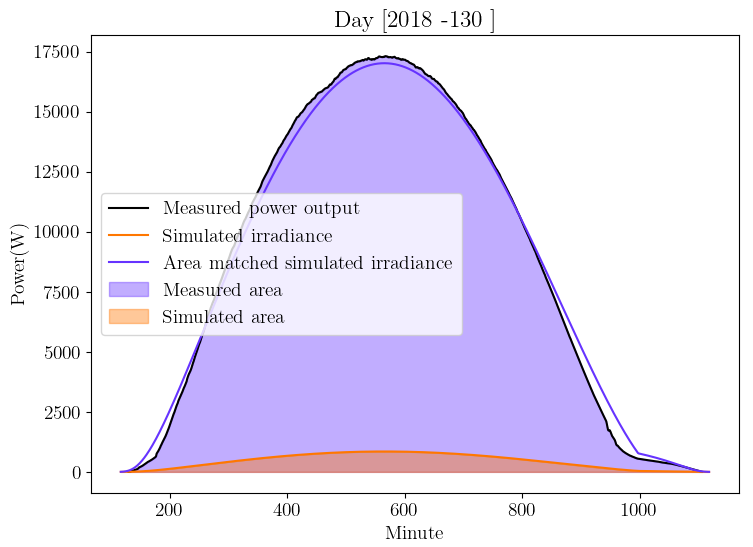
\includegraphics[width=0.7\linewidth]{pics/areamatching2}
\figcaption{Measurement data from FMI Helsinki dataset, POA irradiance simulation was computed with FMI Kumpula coordinates and installation angle parameters.}
\label{fig_area_match}
\end{figure}

\newpage
\subsection{Model improvement results}
The models can be compared with the original measurement data with the following Equation \ref{pv_model_delta}.



\noindent\textbf{Model delta}
\begin{equation}
\begin{split}
\label{pv_model_delta}
Delta_{model} = \sum_{t=0}^{1439} |P_{measured}(t) - P_{simulated}(t)| /1440
\end{split}
\end{equation}

\noindent The $Delta_{model}$ value represents a normalized per minute deviation between the tested model and the measured data. Normalization by division with 1440 results in low delta values as this assumes that the system is constantly generating power regardless of the time of day and thus the resulting delta value is somewhat missleading but for comparison between models these values are still useful.

Delta values for detected cloud free days for FMI Helsinki installation are on average 244W for the POA model and 145W for the improved model based on a sample of 22 cloud free days. For FMI Kuopio the POA model achieved a delta of 487W whereas the delta of the improved model was 320W with a 42 day dataset. This would indicate that the improved PV model is a closer approximation for clear sky PV output than the PVlib POA model.


\begin{figure}[h]
\centering
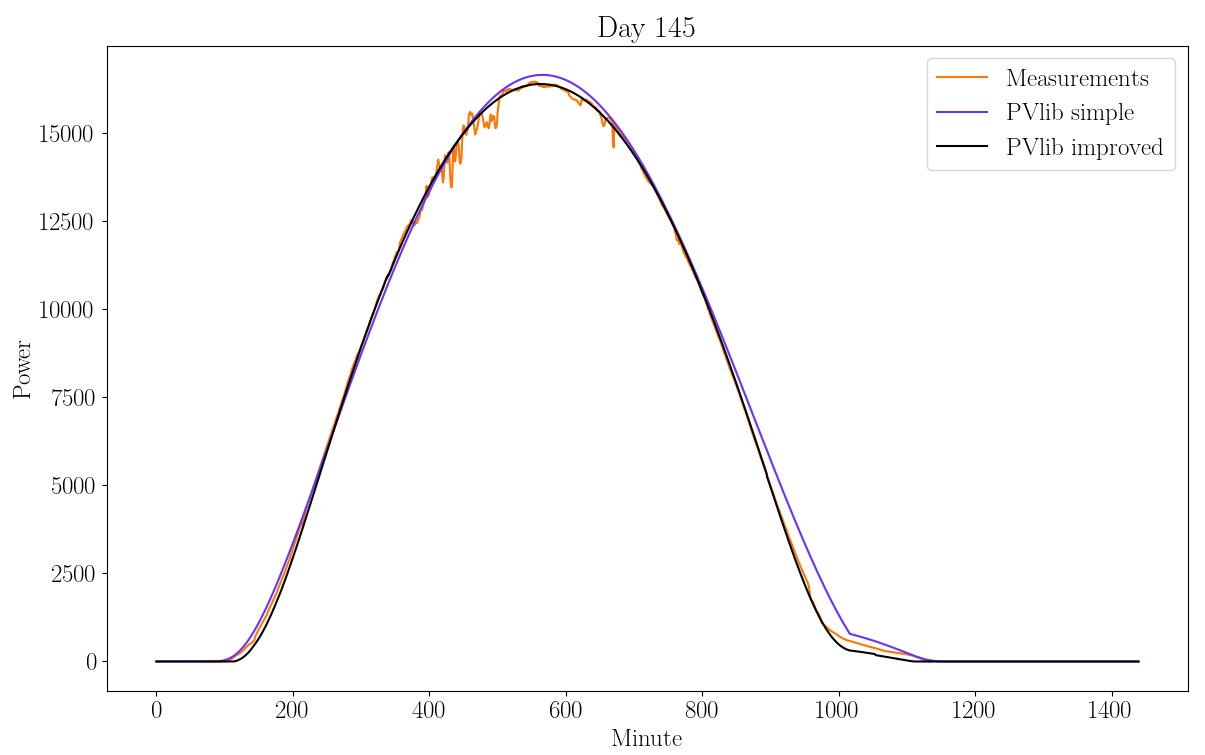
\includegraphics[width=0.99\linewidth]{pics/pvlibsimplecomplex}
\figcaption{Comparison of PVlib POA and the improved PV power generation model on a day from Helsinki dataset.}
\label{fig-poa_eval_simplecomplex}
\end{figure}

\noindent Figure \ref{fig-poa_eval_simplecomplex} shows what the improvement looks like in a best case scenario. The improved model can be seen to approximate the power output with comparable or higher accuracy than the POA model during the tested day. This is especially notable during peak production hours and near 1000 minutes where AOI is high.

Despite the good performance of the improved model, the POA model still has uses due to faster computational speed. If for example only the first and last non-zero minutes matter, it may not make sense to use a physically more accurate model. In the next chapters which of these models is being used will be mentioned on case by case basis.



%that the improved PV model performs better than the simple POA-model at 1000 minutes where the AOI is high and thus reflective losses from direct irradiance are significant. And during peak production minutes where the panel temperatures are likely high enough to cause thermal losses.

%The improved model would appear to be a more accurate approximation for PV generation than the POA model, but the POA model still has uses in applications where faster computation is beneficial or where only the timing of the first and last non-zero minutes matter. Which of these models is being used will be mentioned in the following chapters.

%The model performance could be further tuned as inverter efficiency and other possible factors were not taken into account. However as there are only two datasets, this would increase the likelyhood of overfitting and thus the improved model is left as is.


%is near 90$^\circ$ and during peak production hours where increased temperature effects performance. This is promising but the complexcity of the model also increases the likelyhood of overfitting. Nevertheless this improved model with 2m/s wind speed, 8m elevation and 25 $^\circ$C ambient temperature and the POA model will both be used in the following chapters depending on the charasteristics of parameter estimation functions.

%\noindent Figure \ref{fig-poa_eval_single_day} show that simulations are fairly accurate but there seems to be some deviations between the simulated values and the measurements. The two significant deviations are the noise during peak power generation period and the smooth decrease in power generation during the last hours of the day. The peak power generation noise is likely to be caused by decreases in efficiency due to heat the occasional cooling from gusts of wind. The second deviation between the model and actual measurements is likely to be caused by panel reflections as the south-east orientation of the solar panels results in a high angle of incidence during the last hours of the day.

%Modeling these physical phenomena is possible to an extent if the components of plane of array irradiance are used instead of the POA values. As per Sandia National Laboratories \cite{sandia_poa}, the three components of plane of array irradiance are direct normal irradiance(DNI), global horizontal irradiance(GHI) and diffuse horizontal irradiance DHI. A physically accurate model would compute the absorbed radiation by first projecting the irradiance components to the plane of array adn the estimating the losses caused by reflections. After this is accomplished, the absorbed irradiance could be used to estimate panel temperature and power output.









\chapter{Estimating geographic location}
\label{chapter_est_geoloc}
In order to evaluate the performance of longitude and latitude estimation functions, it may prove useful to be able to translate the error values from degrees to kilometers. The following Equations \ref{equation_latitude_delta_km} and \ref{equation_longitude_delta_km} can be used to approximate the deltas of longitude and latitude estimation functions in kilometers. Note that these functions are only approximations as they rely on the assumption that the Earth is a perfect sphere and not an irregular ellipsoid.


\hfill \break
%%%%%%%%%%%%%%%%%%%%%%%%%%%%%%%%%%%%%%%%%%%%%%%%%%%%%%%%%%%%%%%%%%%%% START
\noindent\textbf{Latitudinal distance to kilometers}(Distance on North-South axis)
%
\begin{equation}
\begin{split}
\label{equation_latitude_delta_km}
Distance_{latitudinal}(lat\_d)=(40 000km/360^\circ)* lat\_d
\end{split}
\end{equation}

\noindent Where 

$lat\_d$ is the distance between two points in degrees latitude.

40000km is an approximation for Earths circumference.

\vspace{5mm} %5mm vertical space
%%%%%%%%%%%%%%%%%%%%%%%%%%%%%%%%%%%%%%%%%%%%%%%%%%%%%%%%%%%%%%%%%%%%% END

%%%%%%%%%%%%%%%%%%%%%%%%%%%%%%%%%%%%%%%%%%%%%%%%%%%%%%%%%%%%%%%%%%%%% START
\noindent\textbf{Longitudinal distance to kilometers at given latitude}(Distance on East-West axis)
%
\begin{equation}
\begin{split}
\label{equation_longitude_delta_km}
Distance_{longitudinal}(lon\_d, lat)=(40 000km/360^\circ)* cos(lat)*lon\_d
\end{split}
\end{equation}

\noindent Where 

$lon\_d$ is the distance in degrees longitude.

$lat$ is the latitude for which the distance is calculated.



\vspace{5mm} %5mm vertical space

\noindent As long as the deviations are small enough and highly accurate error values are not needed, the total error in absolute terms can be estimated by using the latitudinal and longitudinal distances as the x and y coordinates on a cartesian plane and computing the euclidean distance between the origin and resulting point.

%%%%%%%%%%%%%%%%%%%%%%%%%%%%%%%%%%%%%%%%%%%%%%%%%%%%%%%%%%%%%%%%%%%%% END

\newpage
\section{Estimating geographic longitude}
\noindent As mentioned in Sections \ref{section_different_latitudes} and \ref{section_different_longitudes}, the geographic location of a PV system has a strong correlation to the timing of the first and last non-zero measurements of each day whereas the influence of tilt and facing parameters appears to be nonexistent. The relationship would seem to be so clear that without further analysis it would be tempting to use fairly simplistic mathematical models for these estimations. The following longitude estimation Function \ref{equation_naive_longitude} can be derived with two assumptions. These assumptions are that solar noon occurs at 12:00 or 720 minutes at longitude 0$^\circ$ each day and at 6:00 or 360 minutes at 90$^\circ$. Rest of the values can then be linearly interpolated. Note that here solar noon refers to the midpoint between the first and last non-zero minute which is different from astronomical solar noon which occurs nearly at the same time.

As only the first and last non-zero minute times are relevant for longitude and latitude estimation, PVlib POA model is used for both longitude and latitude estimation.

\hfill \break


%The simpler of these relationships is the relationship between the longitude and first and last non-zero minute times. Based on the figure \ref{fig-poa_var_lon2}, this relationship seems to be very close to linear. This makes the use of a simple linear equation rather compelling. 



%%%%%%%%%%%%%%%%%%%%%%%%%%%%%%%%%%%%%%%%%%%%%%%%%%%%%%%%%%%%%%%%%%%%% START

\noindent\textbf{Naive solar noon to longitude equation}
%
\begin{equation}
\begin{split}
\label{equation_naive_longitude}
Longitude(sn)=180^\circ-\frac{360^\circ}{1440}*sn
\end{split}
\end{equation}
Where $sn$ is the approximated solar noon minute calculated by taking the average of first and last non-zero power generation minute of a day. % $0.25$ or $360/1440$ corresponds to the longitude degrees per minute and $180$ is used as offset value. This naive equation assumes that solar noon occurs at 12:00 or 720 minutes each day at $0^\circ$ longitude. Note that here solar noon refers to the midpoint between the first and last non-zero minute which is different from astronomical solar noon which occurs nearly at the same time.

\hfill \break
%%%%%%%%%%%%%%%%%%%%%%%%%%%%%%%%%%%%%%%%%%%%%%%%%%%%%%%%%%%%%%%%%%%%% END


\noindent The simplicity of Equation \ref{equation_naive_longitude} makes the equation appealing, but the assumption of solar noon occuring at 720 minutes should still be verified. In Figure \ref{fig_solarnoons} solar noons can be seen to occur at around 720 minutes at longitude 0$^\circ$ but they can also be observed occuring 15 minutes earlier or later than that. This 15 minute delta would translate into an error range of $(\pm 15/1440)*360^\circ = \pm 3.75^\circ$ degrees or approximately $\pm 200 km$ at the latitudes of Helsinki according to the Equation \ref{equation_latitude_delta_km}.


Knowing that the PV installation is within a 400 kilometer wide slice may in some cases be enough for determining the country in which the PV installation is located in, but for most other purposes this level of accuracy is unlikely to be valuable. Fortunately the naive model can be improved upon by taking the solar noon timing variation into account. \hfill \break

\begin{figure}[ht!]
\centering
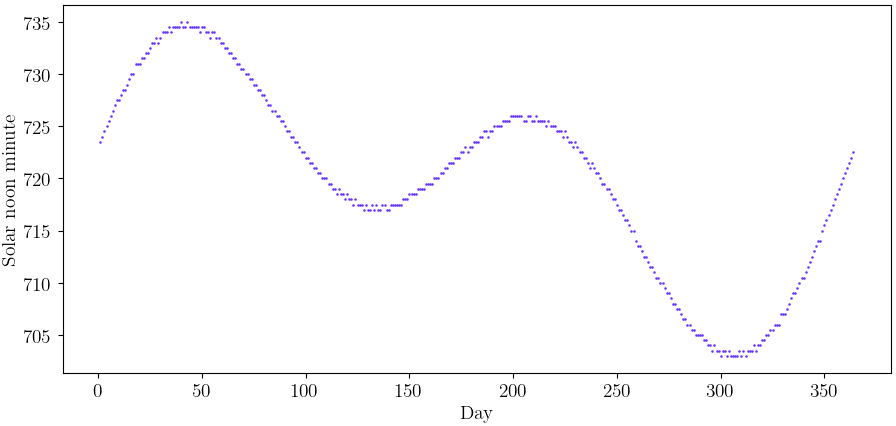
\includegraphics[width=1\linewidth]{pics/solarnoons2}
\figcaption{Approximations of solar noon minutes based on PVlib POA function at longitude $0^\circ$ for year 2023. This pattern is caused by the difference in solar time and UTC time \cite{eot}.}
\label{fig_solarnoons}
\end{figure}



\newpage
%%%%%%%%%%%%%%%%%%%%%%%%%%%%%%%%%%%%%%%%%%%%%%%%%%%%%%%%%%%%%%%%%%%%% START
\noindent\textbf{Improved longitude estimation function }
%
\begin{equation}
\begin{split}
\label{equation_longitude_estimation_2}
Longitude(sn)= \frac{360}{1440}(sn_{poa}-sn)
\end{split}
\end{equation}

\noindent Where $sn$ is the solar noon estimate based on measurement data and $sn_{poa}$ is the simulated solar noon at $0^\circ$ longitude. The new function parameter $sn_{poa}$ compensates for the variation seen in Figure \ref{fig_solarnoons}.


%%%%%%%%%%%%%%%%%%%%%%%%%%%%%%%%%%%%%%%%%%%%%%%%%%%%%%%%%%%%%%%%%%%%% END

\vspace{5mm}


\noindent
%The improved function \ref{equation_longitude_estimation_2} should be much more accurate than the earlier longitude function. as the errors in estimates should primarily be the result of bias in the measurements data.


%In figure \ref{fig_solarnoons_poa_vs_measurement} the solar noon estimates calculated by taking the average of first and last non-zero minute of the day can be seen to preceed the solar noons by roughly 8 minutes. This systematic bias could be explained by the east facing orientation of the panels and correcting for the bias could could be fairly difficult. 

\vspace{0.5cm}
%The theoretical accuracy at this stage could be as high as $\frac{360^\circ}{1440} = 0.25^\circ$ but 
\noindent The improved algorithm should no longer have a systematic error of up to 15 minutes after the difference between solar time and UTC time variation has been taken into account. In addition to correcting for the irregular solar noon timing, the algorithm can be improved even further by using it on larger sections of data and averaging the results, or alternatively, the algorithm could be applied only on selected cloud-free days where the expected errors are likely to be smaller.

If the unfiltered multi-day approach is used, choosing the right day range is crucial. If the range is too narrow, a single outlier value can distort the results significantly, however if the whole year is used, certain periods of the year may contain more noise than others and thus their use could decrease the accuracy of the results. The two scatterplots in Figure \ref{fig_first_last_kuopio_helsinki} show the data quality from the very first and last days of the year seem to be significantly worse than the data from the longest days of the year. Based on these visualizations, days inside the range 100th to 280th would seem best suited for first and last minute sensitive analysis algorithms for both Helsinki and Kuopio installations.



%noise present in non-zero minutes is higher in the Kuopio installation data. 

%noise present in power generation measurements may result in significant errors in estimates based on individual days. These errors can be mitigated by using the algorithm on larger sections of data and averaging the results, or alternatively the algorithm could be applied only on selected cloud free days where the expected errors are likely to be smaller. If the unfiltered multi-day approach is used, choosing the right day range is crucial. If the range is too narrow, a single outlier value can distort the results significantly, however if the whole year is used, certain periods of the year may contain more noise than others and thus their use could decrease the accuracy of the results. The two scatterplots in figure \ref{fig_first_last_kuopio_helsinki} show that the data quality from the very first and last days of the year seem to be significantly worse than the data from the longest days of the year. The same graph would also seem to suggest that overall data quality decreases the further north the installation is. Based on these visualizations, days outside the range of 100th to 280th would seem unsuitable for first and last minute based analysis between latitudes $60^\circ N$ and $63^\circ N$.


\begin{figure}[ht!]
\centering
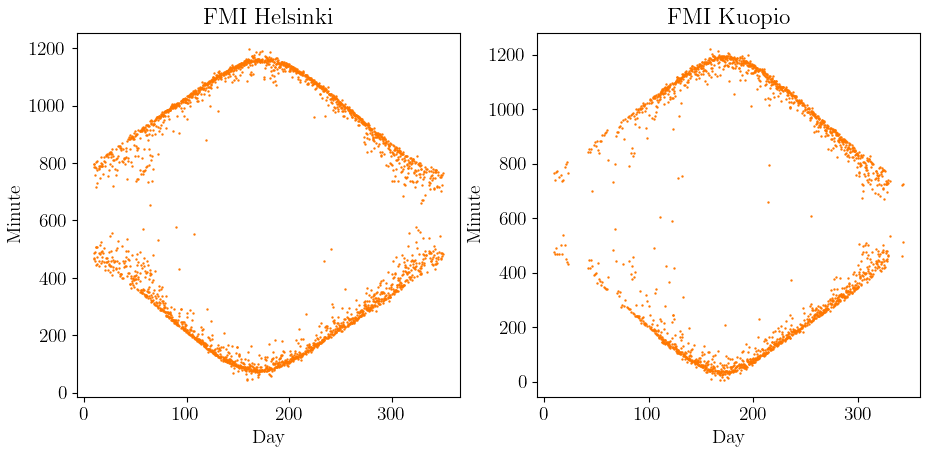
\includegraphics[width=0.9\linewidth]{pics/first_last_helsinki_kuopio2}
\figcaption{First and last non-zero power minutes of each day during years 2017 to 2021 from FMI Helsinki and Kuopio datsets.}
\label{fig_first_last_kuopio_helsinki}
\end{figure}

\clearpage

\subsection{Longitude estimation results}
The longitude estimation algorithm was tested on a day range for each year in the FMI Helsinki dataset and the results are seen in figure \ref{fig_longitude_estimation_helsinki}. By taking the mean of the longitude predictions for each year in the dataset, the resulting longitude estimates varied between -0.804$^\circ$ to 0.0766$^\circ$ from known installation longitudes. Results for the Kuopio dataset shown in \ref{fig_longitude_estimation_kuopio} were similar with mean delta range of -0.1042$^\circ$ to 0.9424$^\circ$.


In kilometers the year with the highest mean deviation of -0.804$^\circ$ in the Helsinki dataset corresponds to an error of approximately 45 kilometers as per \ref{equation_longitude_delta_km}. With Kuopio results the highest delta of 0.9424$^\circ$ is 49 kilometers respectively.

\begin{figure}[ht!]
\centering
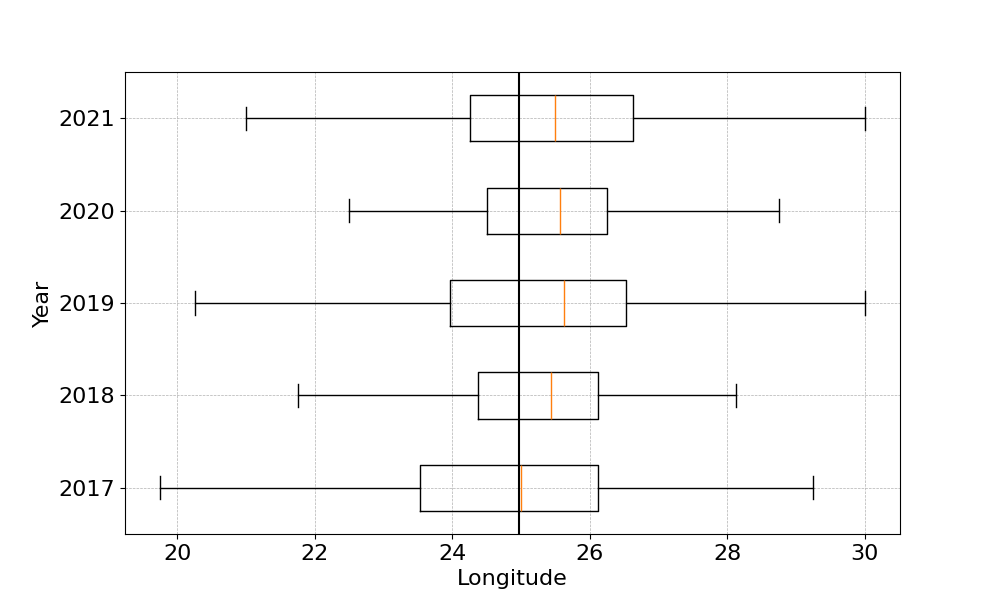
\includegraphics[width=0.9\linewidth]{pics/longitude_v2_helsinki}
\figcaption{Box plot of longitude estimation using FMI Helsinki dataset. Boxes mark 25\% to 75\% quantile intervals and the orange middle lines are the medians. Correct longitude marked as a black line near 25 degrees.}
\label{fig_longitude_estimation_helsinki}
\end{figure}


\begin{figure}[ht!]
\centering
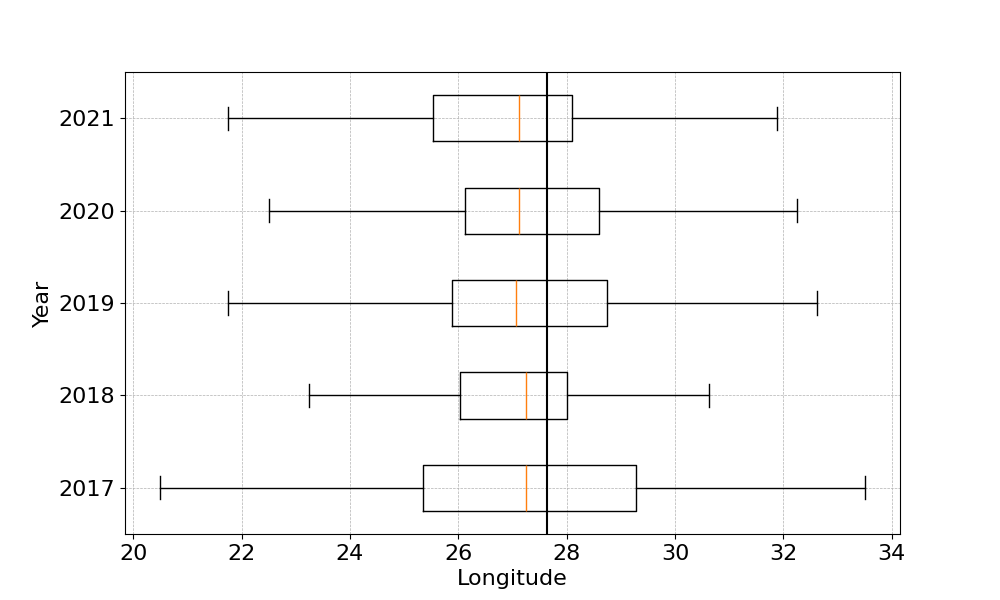
\includegraphics[width=0.9\linewidth]{pics/longitude_v2_kuopio}
\figcaption{Box plot of longitude estimation using FMI Kuopio dataset. Boxes mark 25\% to 75\% quantile intervals and the orange middle lines are the medians. Correct longitude marked as a black line near 25 degrees.}
\label{fig_longitude_estimation_kuopio}
\end{figure}


%The improved algorihm was tested on the day range of 125th to 250th of each year from both FMI datasets and the results can be seen on the Table \ref{table_geolocator_results}. For the Helsinki installations these estimates are all off by less than $0.3^\circ$ while as the Kuopio installation deltas are a bit higher with max of just over $1^\circ$. More impressively, the mean delta of multiple years for the Helsinki dataset is just $0.07^\circ$ and $0.46^\circ$ for Kuopio. In kilometers, the mean deltas can be approximated to 4 and 28 kilometers respectively. The lower accuracy of the Kuopio estimations could be due to multitude of factors ranging from differences in local climate or lower elevation of the installation among others. 




\newpage
\subsection{Possible issues and further development ideas}
While experimenting with the solar minute estimation functions, a curious trait was found. In Figure \ref{fig_solarnoontimes}, the average of the first and last minute is approximately the same for each day at different latitudes as long as the latitude is below 50 degrees. As the latitude is increased, the solar noon estimates begin to deviate significantly, becoming strongly skewed after 70 degrees. 

At first this behavior seems strange as astronomical solar noon should occur happen at the same time when longitude and the day are the same regardless of latitude. However as the solar noon estimates are calculated based on the first and last non-zero irradiance minute of the day, it would make sense that the estimations could be off by significant amount during equinoxes due to rapid changes in day lengths. Measuring out how significantly this affects longitude estimations is challenging. In theory, if the same bias occurs in both the measurements and the model, no corrections would be needed. The effect should be also lessened by using longer day ranges for predicting longitudes or by making sure that the intervals include an equal amount of days from both halves of the year. 

Improvements in the algorithm accuracy could be achieved via by increasing the sampling interval of the irradiance simulations. PVlib POA simulations include a parameter for sampling frequency which is currently set to 1-per-minute in order to match the measuring frequency of FMI datasets. This could be increased to 1-per-second and the added resolution could help in determining more accurate estimates for solar noon times, resulting in possible gains in algorithm accuracy.

PVlib POA model was used instead of the more complex reflection and temperature aware model. This could be done as the geolocation is connected to first and last non-zero minute times which should be the same for both models. However even the POA model might be overly complicated as only two time values are needed.




\begin{figure}[]
\centering
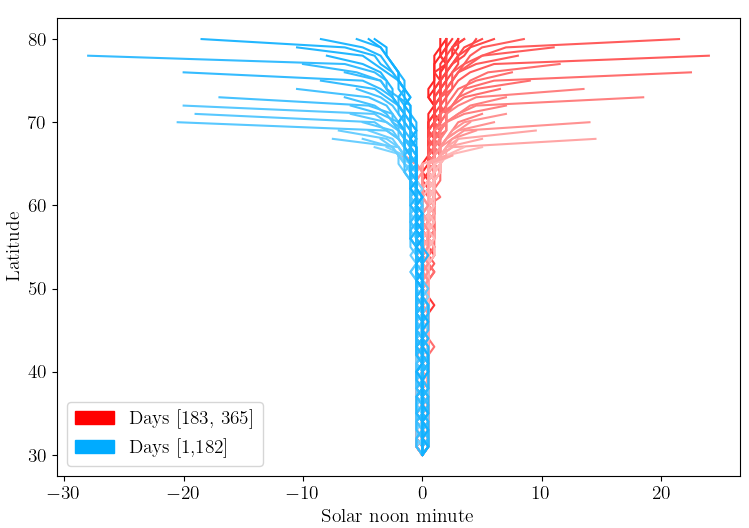
\includegraphics[width=1\linewidth]{pics/solarnoontimes2}
\figcaption{Relationship between latitude parameter and estimated solar noon time. Each line represents a different day of the year and x-axis values are normalized so that each line begins at 0 deviation. Lines with darker colors mark days which are further away from spring and fall equinoxes.}
\label{fig_solarnoontimes}
\end{figure}







%\textbf{Longitude estimation notes}

\newpage 
\section{Estimating geographic latitude}
Similarly to the longitude, the latitude of an installation is strongly connected to the timing of the first and last non-zero minutes of the day. This means that PVlib POA simulations can be used instead of the more complex PV model.

In Figure \ref{fig_poa_var_lat}, the simulated first and last minutes can be seen to change day by day at varying rates based on the latitude. In mathematical terms it could be said that the slope of the day-to-first-minute function is determined by the latitude of the installation. And for the days around equinoxes, and at higher latitudes of $50^\circ$ to $70^\circ$, this relationship would seem to be bijective as per earlier Figure \ref{fig_poa_var_lat}. The followinth algorithm is based on the former observations.


\hfill


\subsection{Latitude algorithm}
%\noindent\textbf{Latitude algorithm}
\begin{enumerate}
  \item Simulate first non-zero minutes over a specific day range at a given latitude.
  
  \item Fit a linear equation to the simulated day to first minute pairs from step 1.
  
  \item Repeat steps 1 and 2 for multiple latitudes and graph the relationship between days and first minutes.
  
  \item Fit a line to the graph from step 3 and save the line slope.
  
  \item Create a slope to latitude graph.
  
  \item Fit an n-degree polynomial equation to the graph from step 5.
  
  \item Calculate the slope of first minutes for real measurement data over the same range as was done in step 1 and use the slope as input for polynomial from step 6. The value of the polynomial is the estimated latitude.
  
\end{enumerate}

\noindent
\textbf{Notes:}
%A visualization of the algorithm can be seen in the following figure \ref{fig_slope_to_latitude}. 
Due to seasonal differences in data quality, polar winters and the midnight sun, the range of days chosen for the algorithm is important. If the range is short, individual outliers in measurements can result in large errors. Whereas if the range is too long, it will be harder to choose the range while avoiding low data quality sections. In the algorithm visualization Figure \ref{fig_slope_to_latitude}, the range of 250th to 300th seems to result in acceptable slope to latitude curve smoothness.
\newpage

%\subsection{Latitude algorithm visualization}
\begin{figure}[ht!]
\centering
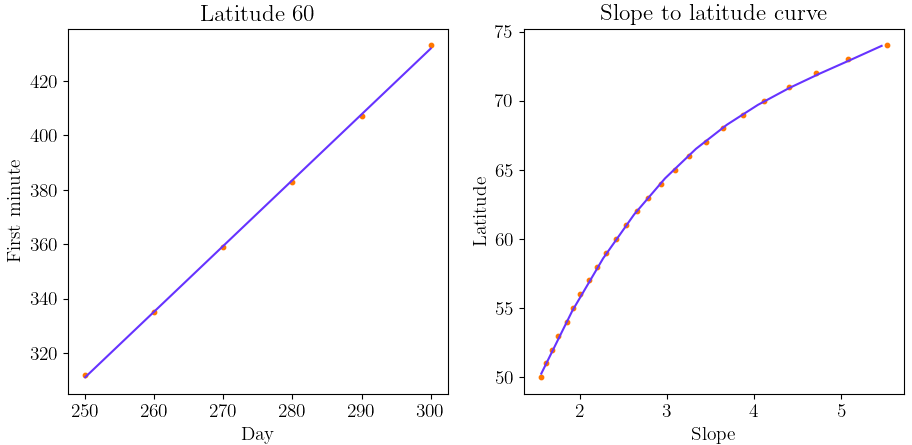
\includegraphics[width=1\linewidth]{pics/slope_to_latitude3}
\figcaption{Left shows the linear relationship between day and simulated first minutes. Right shows the relationship between the slope angle and latitude.}



%the latitude algorithm steps 1 and 2 for day range 250 to 300 at latitude 60 and the linear model fitting. Second graph shows steps 3 and 4 in which slope angles are plotted agains latitudes. The fitted 3rd degree polynomial is $f(x)= 0.305x^3 - 4.607x^2 + 25.953x + 19.908$.}
\label{fig_slope_to_latitude}
\end{figure}



\begin{table}[!ht]
\centering
\begin{tabular}{r|c|c} \hline\hline
 \multicolumn{3}{ c }{FMI Kumpula}\\\hline
Year & Predicted latitude & Error\\
2021 & $61.365^\circ$ &  $1.161^\circ$\\
2020 & $64.493^\circ$ &  $4.289^\circ$\\
2019 & $63.121^\circ$ & $2.917^\circ$\\
2018 & $61.190^\circ$ & $0.986^\circ$\\
2017 & $57.515^\circ$ & $-2.789^\circ$\\


\hline\hline
\end{tabular}
\tabcaption{Results from estimating the latitude of FMI Kumpula PV installation with the preceeding algorithm. Day range of 250th to 300th was used.}
\label{table_geolocator_latitude_results}
\end{table}
\vspace{3mm}
\noindent

\subsection{Improving latitude prediction algorithm}
The results of the algorithm shown in Table \ref{table_geolocator_latitude_results} are somewhere in the correct 


, but the delta of over $4^\circ$ in the 2020 estimate is significant and much higher than the error of the longitude estimation algorithm. The first step in improving the algorithm would be the use of last non-zero minutes as well as the first non-zero minutes. This doubles the amount of outputs from the algorithm and while doubling the amount of outputs does not directly increase the accuracy of the algorithm, it can provide additional insights into the performance of the algorithm. %This is especially valuable as the available datasets are small.



\begin{table}[!ht]
\centering
\begin{tabular}{r|c|c|c|c} \hline\hline

\multicolumn{5}{ c }{FMI Kumpula}\\\hline
Year & First min. p. & Error &  Last min. p. & Error \\
2021 & $61.365^\circ$ &  $1.161^\circ$ & $63.685^\circ$ & $3.481^\circ$\\
2020 & $64.493^\circ$ &  $4.289^\circ$ & $64.288^\circ$ & $4.084^\circ$\\
2019 & $63.121^\circ$ & $2.917^\circ$ & $66.762^\circ$ & $6.558^\circ$\\
2018 & $61.190^\circ$ & $0.986^\circ$ & $60.230^\circ$ & $0.026^\circ$\\
2017 & $57.515^\circ$ & $-2.789^\circ$  & $62.256^\circ$ & $2.052^\circ$\\

\hline\hline
\end{tabular}
\tabcaption{Latitude algorithm with added output for last minutes based prediction.}
\label{table_geolocator_latitude_results_f_and_l}
\end{table}


%Figure \ref{table_geolocator_latitude_results_f_and_l} shows that predictions based on first and last minutes contain similar errors. This is to be expected and it shows that both first and last minutes of each day have similar potetial for latitude estimation. 


\noindent The second step in improving the algorithm is choosing the best possible day range for latitude estimation. One way of choosing the day ranges would be by testing multiple day ranges and choosing the range which results in the lowest average absolute error from the known latitude, but this is problematic as the correct latitude should not be assumed to be known. However if there were multiple datasets with complete metadata, this could be used in order to find universally well-behaving day ranges.

\textit{Standard deviation minimization} is the second option for automated day range selection. As there are two estimated latitude values per year, datasets with $n$ years of data would provide $n*2$ estimated latitude values. Standard deviation of these values could expected to be small if the day interval does not contain days with bad data quality and this means that the interval selection can be automated. Following Figure \ref{fig_heatmap3d2} shows the general shape of the standard deviation plane for FMI Kuopio instalation. 


%However exhaustively searching the day interval space with reasonable intervals can be slow and as seen in the figure \ref{fig_heatmap3d2}, low standard deviation intervals are common in the parameter space. As a result, an arbitrarily chosen long interval is likely to perform almost as well as the very best algoritmicly chosen interval.

%This same figure indicates that an arbitrarily chosen long interval is likely to perform almost as well as the very best algoritmicly chosen interval.


%If the day range is selected well, these estimations could be expected to be tightly grouped. This tight grouping can be measured by calculating the standard deviation and thus the day interval with the lowest standard deviation could be expected to result in the best latitude estimation. A such method relies on the assumption that low standard deviation correlates with good preditions, but this assumption can be shown to be false or missleading. The following figure \ref{fig_heatmap3d2} shows that 

\begin{figure}[]
\centering
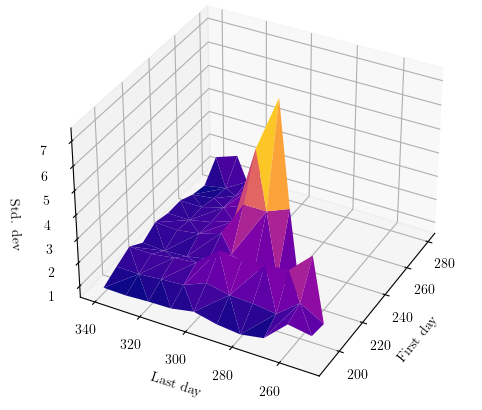
\includegraphics[width=0.5\linewidth]{pics/heatmap3d2}
\figcaption{3D -surface plot of day interval ranges and resulting standard deviations for FMI Kuopio dataset.}
\label{fig_heatmap3d2}
\end{figure}

\newpage

\subsection{Latitude estimation results}
The following two tables contain examples of the results of the latitude estimation algorithm. Results of the latitude estimation algorithm are not as good as the longitude estimations, but for now they will suffice. The predictions follow a similar patter as the previous longitude estimations in that predictions for the Helsinki installation are grouped tighter and their errors are lower than those of the Kuopio installation. 

\begin{table}[!ht]
\centering
\begin{tabular}{r|c|c|c|c} \hline\hline

\multicolumn{5}{ c }{FMI Helsinki latitude estimation results}\\\hline
Year & First min. p. & Error &  Last min. p. & Error \\

2021 & $59.792^\circ$ &  $-0.677^\circ$ & $60.186^\circ$ & $-0.334^\circ$\\
2020 & $59.792^\circ$ &  $-0.412^\circ$ & $60.186^\circ$ & $-0.018^\circ$\\
2019 & $59.896^\circ$ & $-0.308^\circ$ & $59.558^\circ$ & $-0.646^\circ$\\
2018 & $59.945^\circ$ & $-0.259^\circ$ & $59.463^\circ$ & $-0.741^\circ$\\
2017 & $60.577^\circ$ & $0.373^\circ$  & $60.008^\circ$ & $-0.196^\circ$\\

\hline\hline
\end{tabular}
\tabcaption{Estimated latitudes for FMI Helsinki Kumpula dataset with day range of 190th to 250th}
\label{table_geolocator_latitude_results_f_and_l2}
\end{table}

\begin{table}[!ht]
\centering
\begin{tabular}{r|c|c|c|c} \hline\hline

\multicolumn{5}{ c }{FMI Kuopio latitude estimation results}\\\hline
Year & First min. p. & Error &  Last min. p. & Error \\
2021 & $62.626^\circ$ &  $-0.266^\circ$ & $63.197^\circ$ & $0.305^\circ$\\
2020 & $62.259^\circ$ &  $-0.633^\circ$ & $61.895^\circ$ & $-0.997^\circ$\\
2019 & $62.983^\circ$ & $0.091^\circ$ & $62.708^\circ$ & $-0.184^\circ$\\
2018 & $62.722^\circ$ & $-0.170^\circ$ & $62.874^\circ$ & $-0.018^\circ$\\
2017 & $61.669^\circ$ & $-1.223^\circ$  & $61.152^\circ$ & $-1.740^\circ$\\

\hline\hline
\end{tabular}
\tabcaption{Estimated latitudes for FMI Kuopio Kumpula dataset with day range of 190th to 280th.}
\label{table_geolocator_latitude_results_kuopio}
\end{table}

\subsection{Possible issues and further development ideas}
PVlib POA based first and last minute estimations are slower to compute than necessary as only two timestamps are needed. The use of a simpler sunrise and sunset equation would increase the speed significantly, allowing for the use of brute force day range selection algorithms.

Different methods could also be used. In Hagdadi 2017 \cite{navid_australian_article} latitude estimations are done by fitting solar irradiance models with 3 unknown parameters to power generation measurement data. The latitude deltas of 1.65$^\circ$ to 3.42$^\circ$  in the 2017 article are higher than those achieved in this thesis, however as the datasets, geographical regions and algorithms are different, direct comparison can not be made.

%by this paper, however as the datasets, geographical regions and algorithms are different, direct comparison can not be made.

In earlier Figure \ref{fig_slope_to_latitude} the slope to latitude fitting can be seen to be slightly off. This is because the polynomial used is of 2nd degree and higher degree polynomials may result in a closer fit. Similarly a piecewise linear interpolation based fitting could result in a more accurate model and thus better estimation accuracy at the risk of overfitting. 


\newpage
\section{Combined latitude and longitude estimations}
As it is unlikely that the longitude and latitude estimation algorithms are used in isolation from one another, their results should be examined together. This can be done by plotting the estimated locations on a map. Here the two installations in Helsinki and Kuopio and their predicted locations per year are plotted side by side with day range of 190 to 280.

\begin{figure}[h]
	
     \centering
     \begin{subfigure}[b]{0.45\textwidth}
         \centering
         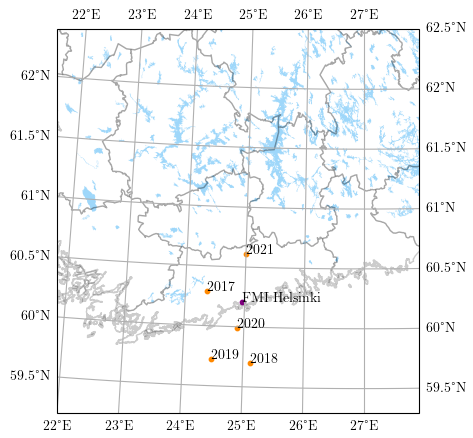
\includegraphics[width=\textwidth]{pics/geolocationmap2}
         \caption{FMI Helsinki.}
         \label{fig_geolocationhelsinki}
     \end{subfigure}
     \hfill
     \begin{subfigure}[b]{0.45\textwidth}
         \centering
         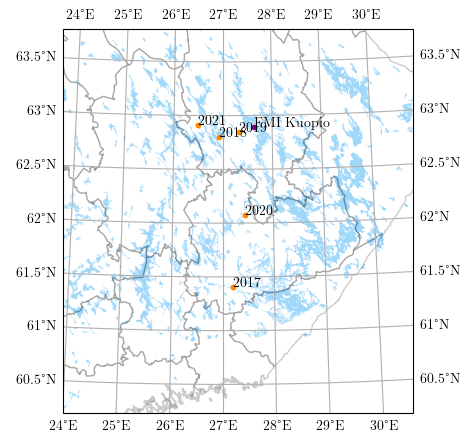
\includegraphics[width=\textwidth]{pics/geolocationmap3}
         \caption{FMI Kuopio.}
         
         \label{fig_geolocationkuopio}
     \end{subfigure}
     \hfill
     \caption{Geolocation estimations for FMI datasets.}
     \label{fig_anglespace}
\end{figure}

\noindent In the Helsinki predictions figure, the estimated geolocations are scattered around the known installation location, showing very little bias and some random noise. Similar behavior can be seen in Kuopio predictions where two outliers 2017 and 2020 deviate more significatly. One degree on the latidue axis is approximately 110 km regardless of latitude and longitude, one degree of longitude is 56km at $60^\circ$ N and 50 km at $63^\circ$ N. As the variance is strongest on the latitude axis, it is likely that the latitude prediction algorithm is more sensitive to variations in the data and further development should be focused on more accurate latitude prediction and day range selection.


The results can be compared to the data resolution. One minute delta in measurements corresponds to a longtudinal shift of 14 kilometers in longitudinal axis at $60^\circ$. As the point cloud width is approximately $1^\circ$ or 50km, the estimates can be thought to have a longitudinal range of 50km, $1^\circ$ or 3.5 minutes with nearly the same values for the Kuopio installation. As the temporal resolution of measurements is 1 minute, the algorithm should not be limited by temporal resolution.
\chapter{Estimating panel angles}
Solar panel installation angles are a large factor in deciding the energy output of a PV system. If panel angles can be freely chosen during planning and installation phases, it can make sense to either optimize for total power generation or power generation during peak consumption hours. This means that even if installation angles could be freely chosen, installation angles are unlikely to be the same for every system in the same geographical region. Panel angles may also be restricted by installation sites and mounting types.

% Panel racks have to be installed based on the available area 

%Installation type also plays a factor in choosing the panel angles. Panel angles may be restricted by 

 %In so called flush rooftop installations, the panels are installed to run along the roof and so the angles can not be freely chosen. Panels can also be rack mounted and these racks tend to be installed and oriented based on the available area as is the case with \ref{fig_fmikumpula_panels}. Due to the forementioned reasons, panel angles vary from installation to installation.

One reason for lacking of faulty metadata is that panel angles can be difficult to measure accurately. The tilt angle of the panels or the angle between the panel normal and zenith(the point directly above) can easily be measured with an angle ruler and a bubble level, but the azimuth angle of the panels is much harder to measure with the same degree of accuracy. If an accurate compass is used and the difference between the magnetic north and the geographic north is taken into account, metal structures and electrical systems nearby can still distort local magnetic fields enough to cause errors in measurements. The challenges in taking accurate measurements are not insurmountable, but they may contribute to the inaccuracies and the lack of available information in PV installation parameter metadata. 

The space of possible panel installation angles can be thought as a half unit sphere in a spherical coordinate system where each point on the surface represents a direction to which the normal of the solar panels could be directed towards. A visualization of parameter space in 3D and 2D is shown in \ref{fig_halfdome} and \ref{fig_anglespace1}. The 3 dots in the subfigure \ref{fig_anglespace1} mark the zenit for which azimuth is not well defined(red), the installation angles of FMI Helsinki installation azimuth $135^\circ$ tilt $15^\circ$(blue) and a close to power generation maximized installation with directly south facing panels with the tilt of $45^\circ$(black).


\begin{figure}[h]
	
     \centering
     \begin{subfigure}[b]{0.35\textwidth}
         \centering
         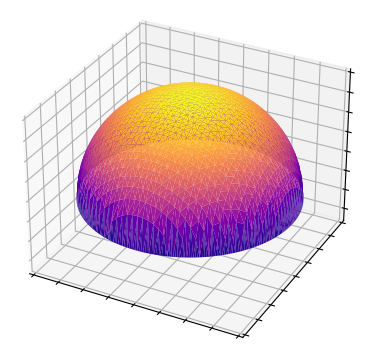
\includegraphics[width=\textwidth]{pics/halfdome}
         \caption{The space of possible angles as a 3D half sphere surface. Each point represents a possible tilt and azimuth combination.}
         \label{fig_halfdome}
     \end{subfigure}
     \hfill
     \begin{subfigure}[b]{0.35\textwidth}
         \centering
         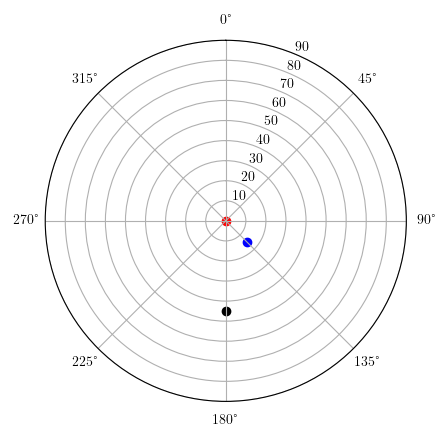
\includegraphics[width=\textwidth]{pics/polarplot}
         \caption{2D projection of the angle space, distance from center denotes the tilt angle of the panels and angle marks the azimuth.}
         
         \label{fig_anglespace1}
     \end{subfigure}
     \hfill
     \caption{Angle space visualizations.}
     \label{fig_anglespace}
\end{figure}


\noindent Estimating panel installation angles requires the use of multiple functions, each of which can be defined in multiple ways. These functions are defined in the following sections.
\begin{itemize}
  \item Prediction error function for quantifying how good a prediction was when the correct panel parameters are known.
  \item Model fitness function for measuring the difference between simulated power values and measured power values.
  %\item Multiplier matching function for matching the magnitude of simulated power values with the magnitude of measurements.
  \item Angle space discretization function for discretizing the angle space into $n$ discrete points which can then be tested with model fitness function.
\end{itemize}




\section{Prediction error function}
%The first part in developing a panel installation estimation algorithm is creating a metric for measuring how well the algorithm performs. 
In this thesis, the proposed error estimation method combines the tilt and azimuth delta values into one error angle value, the angular distance between two points on a spherical surface. The goal is then to develop a panel angle estimation function which achieves the lowest angle error value with the available datasets.

Alternative approaches can also be chosen as the function or functions for measuring the distance between two points in angle space can be defined in multiple ways. The simplest way is to use the delta of known tilt and azimuth angles as two separate error values without normalizing in any way. This method was used in Hagdadi's 2017\cite{navid_australian_article} article but such values are not direcly comparable between installations as the significance of azimuth delta depends on tilt angle.

%Measuring the distance between two coordinate pairs in angle space is more complicated than measuring errors in latitudinal or longitudinal degrees. This difficulty rises from how the azimuth angle lines converge at the pole, resulting in a coordinate system where azimuth delta values are disconnected from the phenomena which they are trying to describe. If the tilt angle is near zero, azimuth delta becomes meaningless but at high tilt angles, even small azimuth delta values can be significant. If this is not corrected for, using azimuth and tilt deltas (changes in angles) as algorithm performance metrics would incorrectly suggest that the data quality of low tilt installations is lower than that of high tilt installations, or that the system is less capable of estimating the parameters of low tilt installations. Due to these reasons, a better way of measuring the distance between two points is needed, luckily the center angle between two points on an unit sphere is easy to solve with geometry and the resulting equation is rather simple.

%While there are no issues with using angles to denote the direction of the panels, the angle values do not map the possible panel angles into the angle space in a way which would make measuring the difference between two angle space coordinates easy. The issues rises from how the azimuth angle lines converge at the pole, resulting in a coordinate system where azimuth delta values are disconnected from the phenomena which they are trying to describe. For example, a 45 degree azimuth delta is fairly significant at tilt of 90 degrees but almost insignificant at 15 degree tilt. If this is not corrected for, using azimuth and tilt deltas (changes in angles) as algorithm performance metrics would incorrectly suggest that the data quality of low tilt installations is lower than that of high tilt installations, or that the system is less capable of estimating the parameters of low tilt installations. Due to these reasons, a better way of measuring the distance between two points is needed, luckily the center angle between two points on an unit sphere is easy to solve with some geometry and the resulting equation is rather simple.

\vspace{3mm}
\noindent\textbf{Deriving angle space distance equation}

\noindent Let $v= [v_1, v_2]$ and $k = [k_1, k_2]$ be two component angle-space vectors so that $v_1$, $k_1$ $\in$ $[0,90]$ and $v_2$, $k_2$ $\in [0,360]$. These vectors represent points on the surface of a unit sphere and their components are the angles of spherical coordinate system. The cartesian coordinates of these points are:
	\begin{align}
	x_v &= sin(v_1)cos(v_2)\\
	y_v &= sin(v_1)sin(v_2)\\
	z_v &= cos(v_1)
  \end{align}
  And
  \begin{align}
	x_k &= sin(v_1)cos(v_2)\\
	y_k &= sin(v_1)sin(v_2)\\
	z_k &= cos(v_1)
  \end{align}
\noindent And the cartesian distance between these two points can be calculated with the following equation:
\begin{align}
	d = \sqrt{(x_v-x_k)^2 + (y_v-y_k)^2+(z_v-z_k)^2}
\end{align}


\noindent The two points and the origin form an isoceles triangle with the sides from the origin to the vector end points having the length of 1 while the distance between the vector end points is the same as d.

\noindent As the lengths of three sides are known, the angles of the triangle can be calculated with the cosine rule. 
\begin{align}
	a^2 &= b^2 + c^2 - 2bc \cos(A)
\end{align}
Where
\begin{conditions}
 a     &  Side opposing the angle A, same as earlier value d \\
 b     &  Side opposing angle B, value is 1  \\   
 c	   &  Side opposing angle C, value is 1
\end{conditions}
\noindent Substituting known values into the cosine equation.

\begin{align}
	a^2 &= b^2 + c^2 - 2bc \cos(A)\\
	d^2 &= 1^2 + 1^2 - 2 \cos(A) \\
	d^2 &= 2 - 2 \cos(A)
\end{align}

\noindent Solving for angle A
\begin{align}
	d^2 &= 2-2\cos(A)\\
	2 \cos(A) &= 2 -d^2 \\
	\cos(A) &= \frac{2-d^2}{2} \\
	A &= \cos^{-1}(\frac{2-d^2}{2})
\end{align}

\noindent Renaming $A$ as $Error$.

\begin{align}
	Error &= \cos^{-1}(\frac{2-d^2}{2}) \label{errorangle}
\end{align}


\noindent By first calculating the distance between the vectors using equations 5.1-5.7 and then substituting the distance into equation 5.16, the resulting angle can then be used as an error value between two panel angle measurements. Python code based on this proof is included in appedix \ref{angular_distace_appendix}.


% This error value is the same as the angle between two points on the surface of a sphere. %In addition, if the deviation occurs only on the tilt axis, the error value and the tilt error are the same.% This makes the error values intuitive.
%In some ways, this method of calculating an error angle is analogous to moving the two angle vectors so that one of them aligns with the 0 tilt point and computing the tilt delta between the two points. Because of this, the error values are fairly intuitive and the error value should better represent the actual difference between installations than other error values calculated via other means.


\vspace{5mm}

%\section{Angle estimation error functions}
%The process of angle estimation requires the use of error estimation functions. The first function is needed for testing the accuracy of the algorithm by translating the known installation angles and the estimated angles into a meaningful error value. This is nontrivial as moving by a set angle value on the tilt and azimuth axis in spherical coordinate space result in different cartesian distances depending on the starting point. 


%The second function or set of functions is needed for evaluating how well a simulated irradiance curve fits the measurement data. Functions of this type can be used for parameter estimation by testing out possible parameter combinations and and choosing the combination which results in the lowest error between the simulated and measured values.


\newpage
\section{Simulation fitness function}
\label{section_simulation_error_function}

The earlier model error function defined in \ref{pv_model_delta} can be re-used as the simulation fitness function. By then computing multiple simulations with different panel angles and choosing the simulation with the best fitness, meaning lowest delta value, the panel angle values can be estimated.

\vspace{6mm}
\noindent\textbf{Simulation fitness function}
\begin{equation}
\begin{split}
\label{pv_model_delta}
Delta_{model} = \sum_{t=1}^{1440} |P_{measured}(t) - P_{simulated}(t)| /1440
\end{split}
\end{equation}

\noindent As the function normalizes delta values by division with 1440, the delta for shorter days is lower than the delta for comparable long days. This should not matter for parameter estimation as the algorithm works by minimizing delta for each day independently. 

Visualization of the function is shown in \ref{fig_simulation_fitness} where simulation with tilt of 90 degrees and azimuth of 135 is tested against known power measurements from a day in FMI Helsinki dataset, resulting in an average delta of 2959.5 W delta per minute.



\begin{figure}[h]
\centering
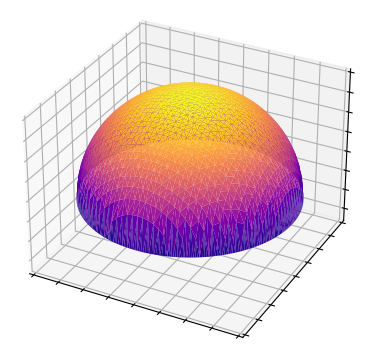
\includegraphics[width=0.8\linewidth]{pics/halfdome} % WAS pics/measured_vs_simulated
\figcaption{Visualization of fitness function.}
\label{fig_simulation_fitness}
\end{figure}




%The earlier simulation error function defined in \ref{pv_model_delta} can be used for evaluating how well a simulated power output curve fits measured power data. By then simulating the power output with several installation parameters and 


%By simulating power generation with different parameter combinations and choosing the set of parameters with the lowest delta value, 



%Simulation error function measures how much the predicted power generation values vary from the measured power generation values. The purpose of the simulation error function is to be able to generate a single numerical value which describes how well a certain parameter combination models the measurements. By then testing out multiple parameter combinations, the combination with the lowest simulation error function value should be the best fit and the parameters used for the simulation should be within a small error of the physical parameters of the solar PV installation. In \ref{fig_error} the error between a cloud free day and randomly chosen set of wrong simulation parameters is visualized.


\newpage
\section{Angle space discretization}\label{angle_space_discretization}
The next step is angle space discretization. The panel angles are denoted with a doublet of tilt and azimuth values, ranging from 0 to 90 and 0 to 360 respectively. If the tilt and azimuth axes are discretized individually in steps of 5 so that tilt is [0, 5, 10, 15... 90] and azimuth [0, 5, 10, 15... 355], the permuations of these tilt and azimuth values create an even grid in the euclidean projection of angle space where x = tilt, y = azimuth. However as the physical phenomena represented by the angle values is not a point on a flat plane but a point on a half-sphere surface, this results in an uneven discretization seen in figure \ref{fig_5step}. 

Sphere discretization problems are relevant for 3D graphics and real world problems involving geometry and so there are pre-existing methods available for discretization. One of the mathematically more elegant methods is the Fibonacci lattice which was used in a similar fashion in González 2009 \cite{Gonzlez}. The mathematical formulation of similar lattices is an older process and an earlier example is found in Vogel 1979\cite{fibolat_old}. The following mathematical notation for the lattice is based on a code sample included in a blog post by Vagner Seibert \cite{medium_fibolat_equation}.




\noindent \textbf{Fibonacci lattice point n of k equation}
\begin{align}
	s &= n + 0.5 \\
	\phi &= acos(1 - 2 s / k) \\
	\theta &= \pi s (1 + \sqrt{5})
\end{align}
Where $n$ is the point number, $k$ is the amount of points, $\phi$ is the panel tilt angle and $\theta$ is the azimuth angle.
\begin{align}
	x &= cos(\theta)sin(\phi)\\
	y &= sin(\theta)sin(\phi)\\
	z &= cos(\phi)
\end{align}
$x$, $y$ and $z$ are the corresponding cartesian coordinates.
\vspace{5mm}


\begin{figure}
     \centering
     \begin{subfigure}[b]{0.45\textwidth}
         \centering
         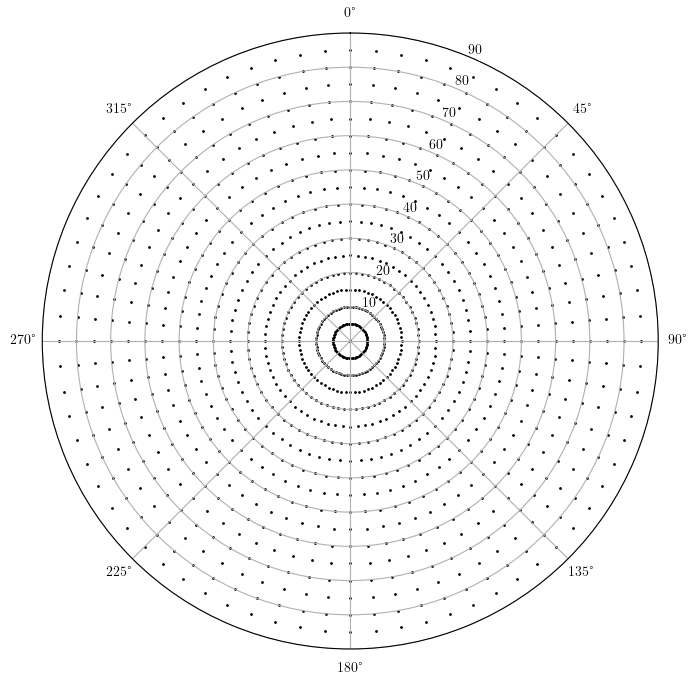
\includegraphics[width=\textwidth]{pics/disc5}
         \caption{In steps of 5 discretization with 1296 points}
         \label{fig_5step}
     \end{subfigure}
     \hfill
     \begin{subfigure}[b]{0.45\textwidth}
         \centering
         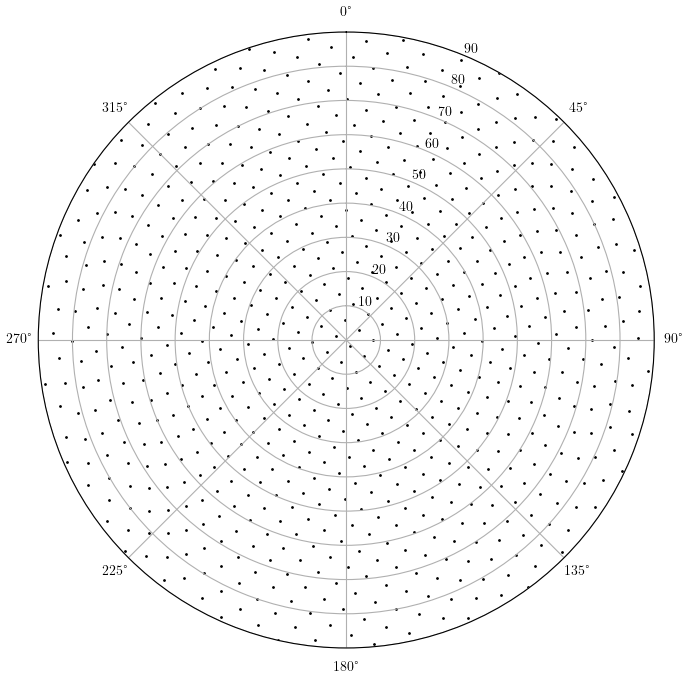
\includegraphics[width=\textwidth]{pics/fibolat1}
         \caption{Fibonacci lattice-based discretization with 756 points.}
         \label{fig_fibolat}
     \end{subfigure}
     \hfill
     
\caption{Comparison of two different discretization patterns. Fibonacci lattice based discretization on right shows a more even distribution of points than the latitude-longitude lattice. The minimum density is approximately the same in both graphs despite the difference in point counts.}
     \label{fig_5stepfibolat}
\end{figure}

\newpage
\subsection{Importance of lattice density}\label{ss_lattice_density}
Using the correct lattice density is important for using exhaustive search algorithms for panel angle estimation. Regardless of the lattice point count, a discrete lattice is unlikely to ever include the best fit in the whole $\mathbb{R}^2$ parameter subspace. This means that if the lattice density is low, distance between best fit and closest lattice points can result in significant errors. However as incresing the lattice density increases the computational cost of angle estimation, choosing a good density is an optimization problem.

With \textit{in-steps-of-n} lattices, the main benefit is easy readibility. If the lattice is given one point for latitudinal and longitudinal degree, resulting in $360*90=32400$ points, then the lattice can be aligned so that each tilt and azimuth degree pair where angles are integers is tested. This discretization makes the results easily understanble as if the known installation angles are given as integers, a point representing the exact known installation angles already exists on the lattice. The same applies for lower density in \textit{in-steps-of-n} lattices.

If a Fibonacci lattice or some other discretization method where lattice points do not fall on angle space integer grid lines is used, evaluating the performance of the fitting algorithm can become somewhat challenging. For example a 1000 point Fibonacci lattice with a delta of 5 degrees is not as descriptive of a result as a delta of 5 degrees on a 1 degree \textit{in-steps-of-n} lattice.


%The density of lattices is an important measurable charasteristic which proves useful during the optimization of angle estimation algorithm. The most useful metric would be the sphere center angle distance between neighboring points. This would be useful as it can be used for determining whether errors in predictions are lattice or function fitting related. For example, if the lattice neighbors are approximately 1 degree away from oneanother and the predicted angle is 5 degrees off from the known installation angle, then the error is caused by model fitting and not lattice density as there must have been multiple lattice points closer to the known angle point than the discovered best fit. However if grid density is near to or lower than angle estimation error, the lattice is likely to be a contriburing to angle estimation errors.

%Calculating neighborign center angle distances for both \textit{in-steps-of-n} and Fibonacci lattices is somewhat challenging. In \textit{in-steps-of-n}, the value \textit{n} can be used as an estimate for max center angle distance as \textit{n} will always be the tilt distance to the nearest neighbor with different tilt angle. With Fibonacci lattices the easiest way of estimating center angle distances is taking the coordinates of the first two lattice points and calculating their center angle distance with earlier error equation \ref{errorangle}. These first two points should be used as Fibonacci lattice points are distributed on a single arm spiral pattern, resulting in later sequential points being further from one another.

%Another method for calculating Fibonacci lattice point distances is dividing the surface area of the angle space by the amount of calculated lattice points. This area-per-point value could then be used in order to estimate how far points are from oneanother on average. In later sections, the first two points derived distance will be used.

\newpage
\section{Solving panel angles}
Now that the geographic location and multiplier value of installation are known to be solvable and fitness functions have been defined, the next step is solving the panel angles. The simple method is evaluating all points on a sufficiently dense lattice and choosing the point with the lowest delta value.

Figure \ref{fig_polar10} contains 10 fibonacci lattice points and their normalized delta values. The best fit was at tilt 31.79$^\circ$, azimuth 153.79$^\circ$ and it had a delta value of 369W. The lattice density leaves large gaps between lattice points and this found best fit is the closest point to the known installation angles of 15$^\circ$ and 135$^\circ$. Center angle error as per \ref{errorangle} is 18.17$^\circ$.




%is to solve the panel installation angles. The chosen method relies on splitting angle space into $n$ discrete points and evaluatin each of their fitness by calculating an error value. Here the angle space was split into 10 discrete points with fibonacci lattice \ref{angle_space_discretization} and the fitness of each point was evaluated with area error \ref{areaerror} and multiplier matching \ref{function_multipliermatch} functions. %The tilt-azimuth pair with the lowest error value was 31 


\begin{figure}[h]
\begin{floatrow}
\ffigbox{%
  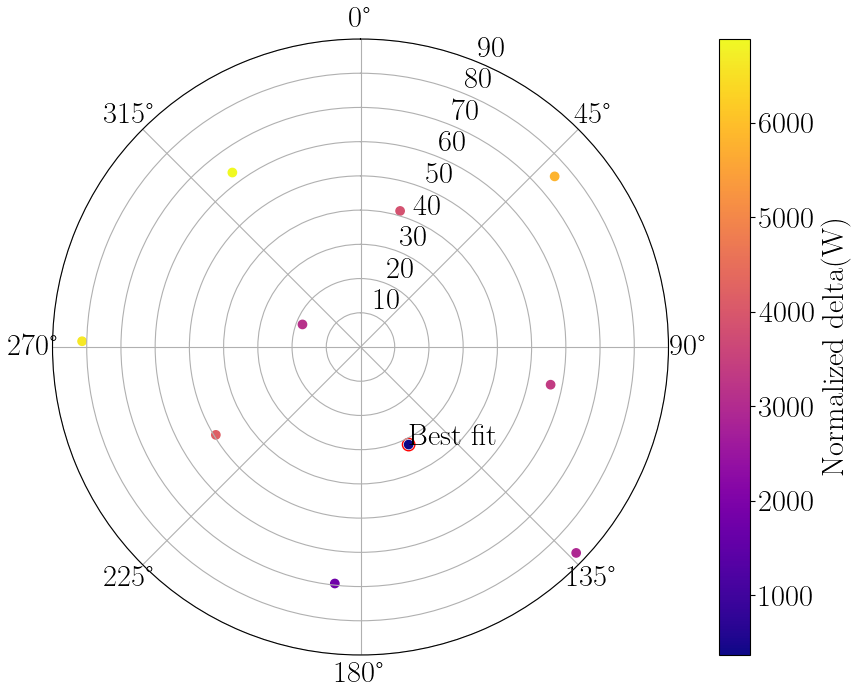
\includegraphics[width=1\linewidth]{pics/10p_fibo_fit_text} % WAS pics/10p_fibo_fit_text
}{
  \caption{Polar plot of test points for a single day of data from FMI Kumpula dataset.}
  \label{fig_polar10}
}
\capbtabbox{%
  \begin{tabular}{c|c|c} \hline

Tilt$^\circ$ & Azimuth$^\circ$ & Delta(W)\\
\hline
18.19 & 291.25 & 3128\\
\textbf{31.79} & \textbf{153.74} & \textbf{369}\\
41.41 & 16.23 & 3873\\
49.46 & 238.72 & 4183\\
56.63 & 101.22 & 3356\\
63.26 & 323.71 & 6888\\
69.51 & 186.2 & 1759\\
75.52 & 48.69 & 5814\\
81.37 & 271.18 &  6626\\
87.13 & 133.68 & 2938\\
\hline\hline
\end{tabular}
}{%
  \caption{Tilt, azimuth and error table for single day.}
}
\end{floatrow}
\end{figure}

The fit achieved in \ref{fig_polar10} is not very good and better results can be achieved by increasing the lattice density. The trivial method is to use a fibonnacci lattice with a higher point count, for example the fit achieved with a 10 000 point lattice \ref{10k_fits_new_helsinki} found the best fit at tilt 14.79$^\circ$, azimuth 136.2$^\circ$ , delta value of 136.2W and center angle error of 0.3659 degrees$^\circ$. This is a much better fit but increasing the lattice density comes with a higher computational cost. Depending on code optimizations, evaluating a single day from the dataset against a 10 000 point lattice can from a minute up to several hours.

\begin{figure}[h]
\centering
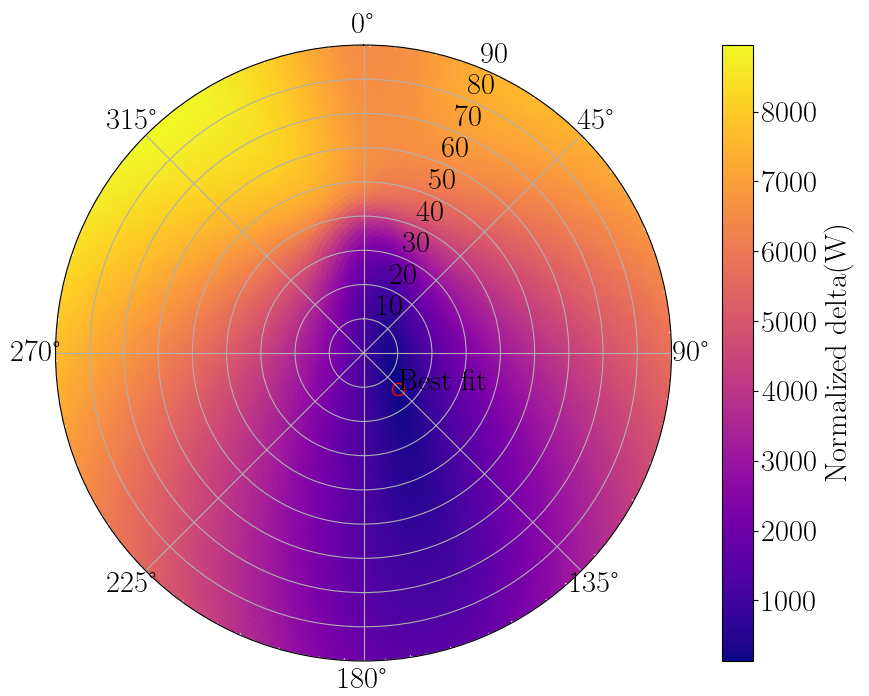
\includegraphics[width=0.8\linewidth]{pics/10k_new_model} % WAS pics/measured_vs_simulated
\figcaption{Results of a 10 000 datapoint lattice fitting against a single day from FMI Helsinki dataset. Center angle error between the found best fit and known installation angles is 0.3659$^\circ$.}
\label{10k_fits_new_helsinki}
\end{figure}



%# Best fit was tilt: 14.79 azimuth: 136.2 fitness:133.3 10k lattice result !






%\noindent Now that the method can be seen to work, it is time to improve the results. This can be done by generating larger lattices and thus by evaluating higher amount of datapoints, the algorithm has a higher chance of finding the global minimum error point. As per \ref{ss_lattice_density}, Fibonacci lattice of 1000 points would have the angular resolution of approximately 4 degrees where as 10000 points would be near to 1.5 degrees. The performance can also be improved by evaluating best fits for multiple days at once. The resulting point cloud of best fits can then be used for averaging out noise in the predictions.

%The plot \ref{fig_polar_multiyear} is a result of using the angle finding algorithm on 41 days from FMI Kumpula dataset with a Fibonacci lattice of 1000 points. The two darker spots near the center of the graph are the two most common best fits, [17.0$^\circ$, 138.4$^\circ$] with 17 and [22.7$^\circ$, 143.1$^\circ$] with 16 out of 41 days. These groupings are as close to the known installation angles of [15$^\circ$,  135$^\circ$] as could be expected from a 1000 point lattice. The next step is tightening the cluster, this can be done by adjusting the smoothness requirement of the cloud free day algorithm or by restricting the day range. In \ref{fig_polar_multiyear_summer} the tightening was accomplished with day range restrictions and 22 days were accepted by the algorithm.


%In \ref{fig_polarplot_13days} the polar plot is a result of taking the 13 best days from FMI Kumpula dataset year 2018 and using a fibonacci lattice with 500 test points. The most common best fit was [27.5$^\circ$, 150.8$^\circ$] with 5 occurances followed by [24.1$^\circ$, 138.4$^\circ$] with 4 days. These values are close to the 





%As all of the estimates converge on two neighboring points, the final step is increasing the lattice resolution further. With 10 000 point lattice, the cluster tightened further \ref{fig_polar_multiyear_helsinki10k}. Out of the 22 days, 7/22 or 32\% had best fit at [19.34, 136.87] with error of 4.38 degrees and 6/22 or 27\% at [17.74, 135.06] with error of 2.74 degrees. Rest of the best fits were distributed in smaller clusters near these points. The lowest angle distance best fit was [17.09, 130.32] with angle distance of 2.46 degrees. As the angle distance errors are higher than the discretization resolution and as the predicted angles are systematically biased, it would seem that the error is caused by the solar irradiance model or model fitting and not angle space discretization.


%As the angle distance errors are higher than the discretization resolution and as the results seem biased, the errors of the estimation algorithm would seem to be caused by inaccuracies in model fitting and not angle space discretization.




%\begin{figure}[h]
%\centering
%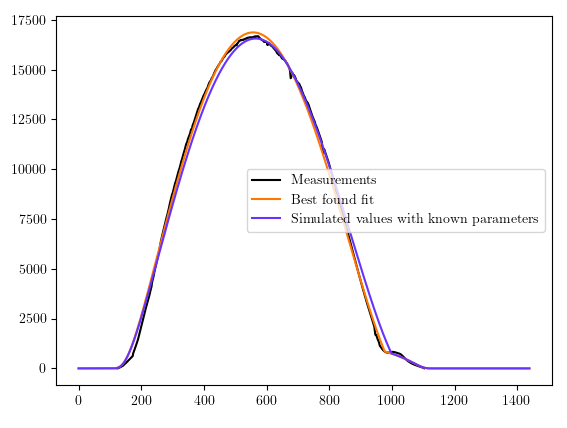
\includegraphics[width=0.8\linewidth]{pics/10kfitshelsinkiplot}
%\caption{Comparison between measured values, simulated values with known installation parameters and best found fit.}
%\label{fig_10kfitshelsinkiplot}
%\end{figure}



%day 141 predicted 17.74 135.06 delta degrees: 2.74 x
%day 145 predicted 19.92 141.6 delta degrees: 5.3
%day 148 predicted 19.34 136.87 delta degrees: 4.38 	x
%day 179 predicted 17.74 135.06 delta degrees: 2.74 x
%day 197 predicted 21.37 143.41 delta degrees: 6.87 y
%day 198 predicted 18.37 139.79 delta degrees: 3.64
%day 199 predicted 19.34 136.87 delta degrees: 4.38		x
%day 157 predicted 19.92 141.6 delta degrees: 5.3
%day 169 predicted 18.37 139.79 delta degrees: 3.64
%day 202 predicted 17.74 135.06 delta degrees: 2.74 x
%day 208 predicted 21.37 143.41 delta degrees: 6.87 y
%day 143 predicted 19.34 136.87 delta degrees: 4.38		x
%day 155 predicted 19.92 141.6 delta degrees: 5.3
%day 164 predicted 19.92 141.6 delta degrees: 5.3
%day 166 predicted 17.74 135.06 delta degrees: 2.74 x
%day 171 predicted 19.34 136.87 delta degrees: 4.38		x
%day 174 predicted 17.09 130.32 delta degrees: 2.46
%day 175 predicted 17.74 135.06 delta degrees: 2.74 x
%day 177 predicted 17.74 135.06 delta degrees: 2.74 x
%day 178 predicted 19.34 136.87 delta degrees: 4.38		x
%day 179 predicted 19.34 136.87 delta degrees: 4.38		x
%day 200 predicted 19.34 136.87 delta degrees: 4.38		x



%day 145 predicted 32.09 196.89 delta degrees: 18.65 x
%day 192 predicted 30.5 198.01 delta degrees: 16.96 y
%day 199 predicted 30.5 198.01 delta degrees: 16.96 y
%day 210 predicted 34.52 197.58 delta degrees: 20.9 z
%day 212 predicted 32.09 196.89 delta degrees: 18.65 x
%day 213 predicted 35.07 194.65 delta degrees: 21.86 k
%day 167 predicted 27.07 200.24 delta degrees: 13.37 i
%day 143 predicted 30.5 198.01 delta degrees: 16.96 y
%day 144 predicted 28.83 199.13 delta degrees: 15.21 l
%day 145 predicted 28.83 199.13 delta degrees: 15.21 l
%day 162 predicted 27.07 200.24 delta degrees: 13.37 i 
%day 167 predicted 27.07 200.24 delta degrees: 13.37 i 


\newpage
\subsection{Evaluation of exhaustive search results}
The results of the exhaustive search algorithm are good for the Helsinki dataset. Angle delta values as low as achieved in \ref{10k_fits_new_helsinki} are likely to be irrelevant for analysis purposes and a delta of 0.37$^\circ$ is lower than the single digit precision of reported installation angles.

The next verification step is using the algorithm on multiple days from the same dataset and checking the spread pattern. This was done for a set of days from 2018 and 2020, resulting in scatter patterns shown in \ref{fig_fmi_helsinki_1000_multi_day_2018} and \ref{fig_fmi_helsinki_1000_multi_day_2020}. The tight clustering visible in both figures suggest that the  



%By using the same method and plotting the best fits for several cloud free days from one dataset, the found best fits cluster tightly around the known installation angles as seen in figures \ref{fig_fmi_helsinki_1000_multi_day_2018} and \ref{fig_fmi_helsinki_1000_multi_day_2020}. The years 2018 and 2020 were chosen for higher number of days passing the set cloud free day selection threshold.


\begin{figure}[!h]
\begin{floatrow}
\ffigbox{%
  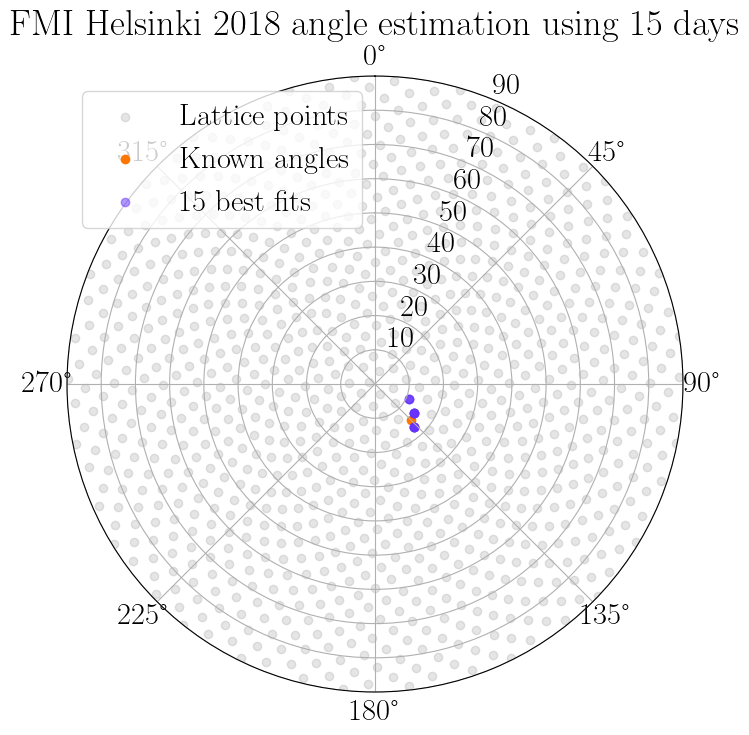
\includegraphics[width=1\linewidth]{pics/FMI_helsinki_2018} % WAS pics/10p_fibo_fit_text
}{
  \caption{1000 point exhaustive search on 15 cloud free days from FMI Helsinki dataset using year 2018.}
  \label{fig_fmi_helsinki_1000_multi_day_2018}
}

\ffigbox{%
  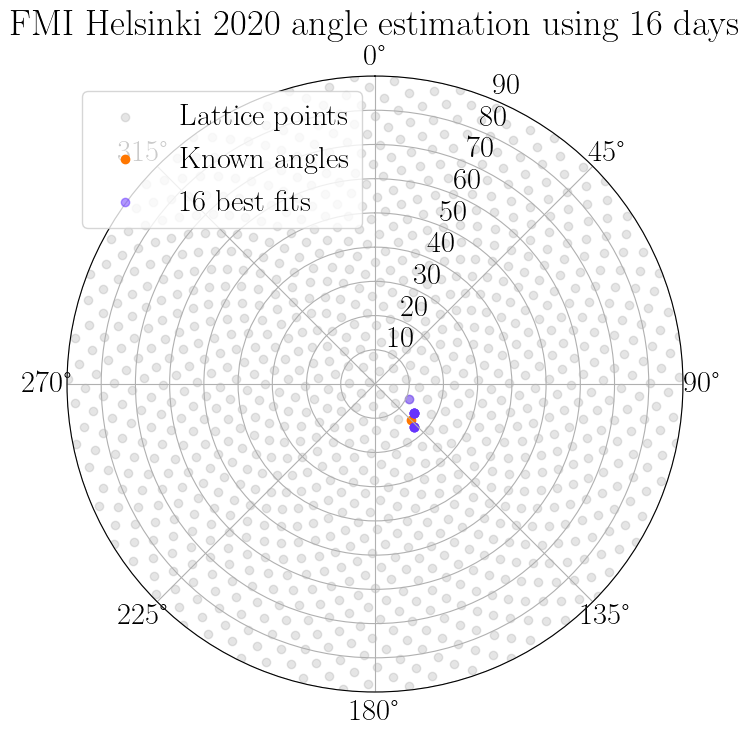
\includegraphics[width=1\linewidth]{pics/FMI_helsinki_2020} % WAS pics/10p_fibo_fit_text
}{
  \caption{1000 point exhaustive search on 16 cloud free days from FMI Helsinki dataset using year 2020.}
  \label{fig_fmi_helsinki_1000_multi_day_2020}
}
\end{floatrow}
\end{figure}

Results for the Kuopio dataset are not nearly as good as the Helsinki predictions. Figures \ref{fig_fmi_kuopio_10000_multi_day_2017} and \ref{fig_fmi_kuopio_1000_multi_day_2018} clearly indicate that estimations are converging several degrees off from the known installation angles. In the more dense 10000 point lattice used for the year 2017 the mean of tilt and azimuth predictions is 26.76$^\circ$ and 201.11$^\circ$, resulting in a center angle delta of 13$^\circ$. 

The exact reason for this significant delta is not known and there could be multiple contributing factors. One possible explanation is panel shading which is more likely to occur when the Sun is near the horizon. This causes a proportionally higher energy output loss during first and last hours of the day, resulting in a more narrow power generation plot shape. This \textit{sharpness} is also influced by the tilt angle of an installation as was previously seen in figure \ref{fig_poa_different_parameters} and thus the error in the estimated tilt angle could be partially caused by either panel self shadowing or shadowing caused by other stuctures near the PV panels.

Similar patterns occur with all of the years from FMI Helsinki and Kuopio datasets where estimated angles form clusters in angle-space. With Helsinki the delta between known installation angles and estimations is minimal where as with the Kuopio dataset the cluster is larger and offset by a bias of approximately 13$^\circ$.


%average delta angle: 12.956
%Average tilt:26.76 azimuth:201.11 fitness290

\begin{figure}[h]
\begin{floatrow}
\ffigbox{%
  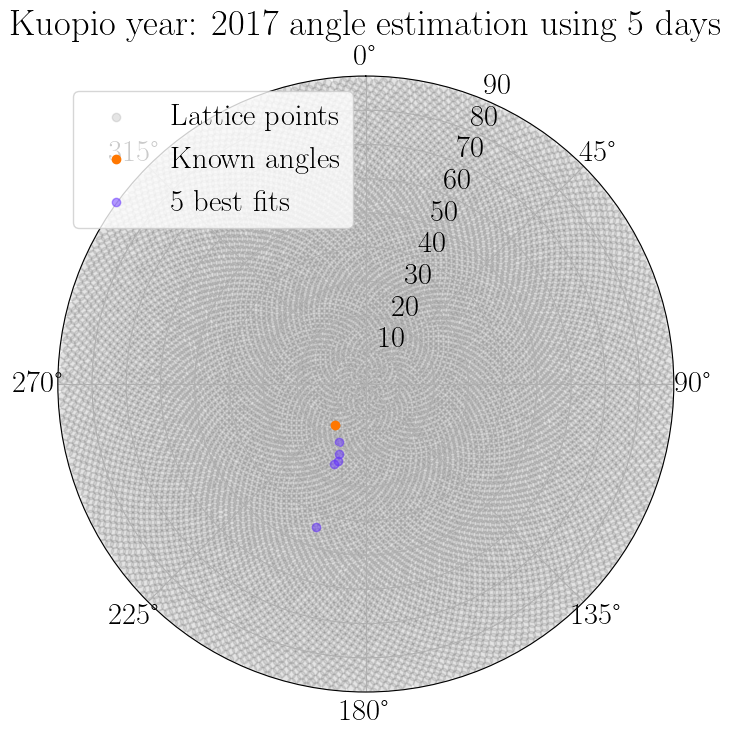
\includegraphics[width=1\linewidth]{pics/Kuopio2017} % WAS pics/10p_fibo_fit_text
}{
  \caption{10000 point exhaustive search on 5 cloud free days from FMI Kuopio dataset using year 2017.}
  \label{fig_fmi_kuopio_10000_multi_day_2017}
}

\ffigbox{%
  \includegraphics[width=1\linewidth]{pics/FMI_kuopio_2018} % WAS pics/10p_fibo_fit_text
}{
  \caption{1000 point exhaustive search on 18 cloud free days from FMI Kuopio dataset using year 2018.}
  \label{fig_fmi_kuopio_1000_multi_day_2018}
}
\end{floatrow}
\end{figure}


\newpage

\section{Solving panel angles iteratively}
The exhaustive search used in earlier section suggest that the method is capable of estimating panel installation angles accurately. However evaluating 10 000 point lattices is somewhat inelegant and this can be avoided by using multiple less dense lattices iterarively if the fitness space satisfies some requirements.

The first requirement is that the fitness space should be smooth. This smoothness doesn't have to be perfect, fine patterns and details in the fitness space surface do not cause issues with iterative search algorithms if the noise pattern is not observable in the iterative lattices. Based on an earlier figure generated by exhaustive search \ref{10k_fits_new_helsinki}, this requirement would appear to be met.

Second requirement is that the fitness space should contain as few convergence points and their respective basins as possible. These basins are regions in fitness space which are defined by a convergence point and their surrounding regions where the slope of the space leads to the respective convergence point. The region around best found fit in \ref{10k_fits_new_helsinki} forms a large basin but there would also appear to be a second converge point at azimuth 0$^\circ$ tilt 90$^\circ$.

 

\noindent \textbf{Iterative panel angle estimation algorithm}
\begin{enumerate}
	\item Choose a cloud free day from the dataset for evaluation.
  \item Choose a starting or "center" point from the angle space. This can be either the best result from a low density lattice or a fixed point such as tilt 45$^\circ$ azimuth 180$^\circ$.
  \item Evaluate the fitness at the center point and store that as the center point fitness.
  \item Choose a few points near this center point within a given distance and evaluate their fitness. If any of the neighboring points results in a better fit than the center point, this point will then be chosen as the new center point.
  \item Repeat steps 3 and 4 until step 4 does not find a better fit. When this happens, decrease the distance used for the local lattice in step 4.
  \item Repeat steps 3,4 and 5 for a set number of times. Last center point is the best iteratively found fit.
\end{enumerate}


\noindent Step 4 is the first non-trivial step in the algorithm. The selection of neighboring points can be done in multiple ways, the cross pattern search method shown in figure \ref{fig_iterative_visual_1} is based first transforming the starting angle tilt 45$^\circ$  and azimuth 270$^\circ$ to a cartesian coordinate plane point and the generatin 4 nearby cartesian plane points at distance of 0.3 which are then transformed back into angle space. The equations used for space transformations are \ref{angle_space_to_unit_circle} and \ref{unit_circle_to_angle_space}. This space transformation method results in visually pleasing plots and the cartesian distance of 0.3 is easily adjustable in step 5 of algorithm.

\newpage

\noindent \textbf{Unit circle to angle space equations}

\begin{equation}
\begin{split}
\label{unit_circle_to_angle_space}
d &= x^2+y^2\\
Tilt &= \sqrt{d}*90^\circ\\
Azimuth &= tan^{-1}2(x/d, y/d)
\end{split}
\end{equation}

\noindent \textbf{Angle space to unit circle equations}
\begin{equation}
\begin{split}
\label{angle_space_to_unit_circle}
d &= Tilt/90^\circ \\
x &= cos(Azimuth)d \\
y &= sin(Azimuth)d \\
\end{split}
\end{equation}

\vspace{5mm}





\begin{figure}
     \centering
     \begin{subfigure}[b]{0.45\textwidth}
         \centering
         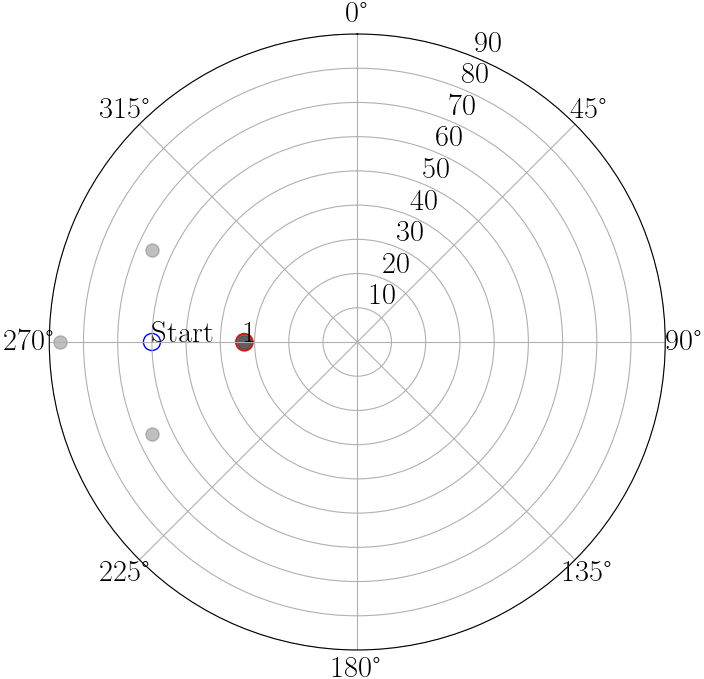
\includegraphics[width=\textwidth]{pics/iterative_1_step}
         \caption{Iterative best fit search after 1 cross pattern search.}
         \label{fig_iterative_1_step}
     \end{subfigure}
     \hfill
     \begin{subfigure}[b]{0.45\textwidth}
         \centering
         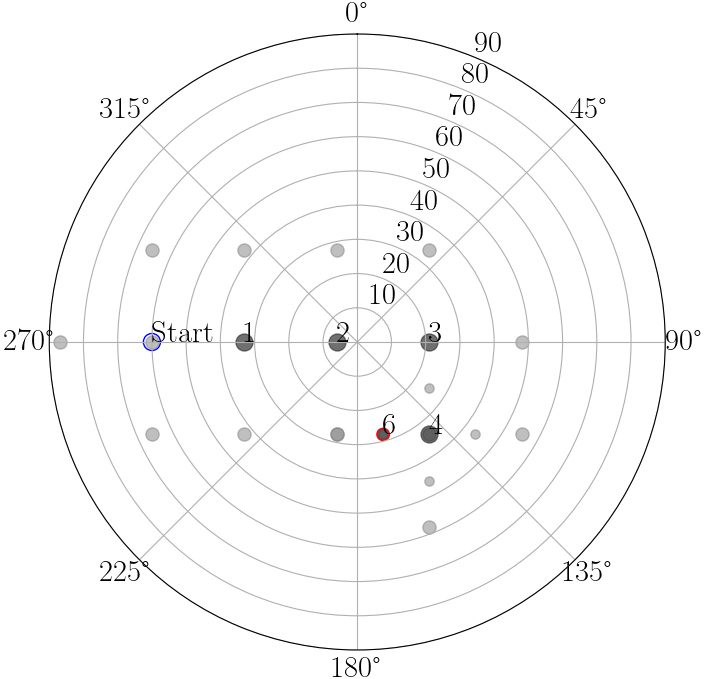
\includegraphics[width=\textwidth]{pics/iterative_6_step}
         \caption{Iterative best fit search after 6 cross pattern searches.}
         \label{fig_iterative_6_step}
     \end{subfigure}
     \hfill
     
\caption{Visualization of iterative best fit search algorithm. Numbers next to markers indicate that a point was the best found during n:th cross pattern search. Number 5 is missing from \ref{fig_iterative_6_step} as no new best fit was found, resulting in search distance deacrease. Red circle marks the best found fit.}
     \label{fig_iterative_visual_1}
\end{figure}









\chapter{Conclusion}
PV system parameter estimation results for the FMI Helsinki dataset are very good to excellent. Angle estimation results with a center angle delta of less than 1$^\circ$ were achievable with both iterative and exhaustive algorithms. Geolocation estimation proved to be more difficult with the scatter pattern from multiple years having small amount of bias and a fair amount of noise. Scatter formation is spread around the FMI Helsinki installation and is approximately 50km by 200km in dimensions. Due to small sample size of 5 datapoints this algorithm is harder to evaluate.

Results for FMI Kuopio dataset were noticeably worse. Center angle delta with panel installation angles was approximately 13$^\circ$ regardless of estimation method used. Similarly the scatter pattern in geolocation estimation resulted in a 50km by 300km region with outliers.

The differences in the algorithm performances between the datasets can partially be explained by the noise present in the Kuopio data where something would appear to be casting shadowns onto the panels. Differences may also be partially caused by parameter estimation algorithm parameters such as used day ranges which affect the results of estimation algorithms.




%The initial goal of this thesis was to find a simple way of estimating parameters of solar PV installations and this goal has been accomplished with moderate success. Some of the algorithms are thousands of lines of long, but the underlying mathematics was still kept relatively simple. As a result, the code can be understood and modified by a wider audience.

%From the perspectives of mathematics and programming, model fitting problems are not particularly difficult. In this thesis, the challenges rose from optimization, understanding patterns in the data and discovering where the limits of the estimation algorithms come from. The insights gained while tackling these issues may be more valuable in to other researchers than the final estimation algorithms.





%The most significant of which are the center angle error function, Fibonacci-lattice based angle space discretization and angle space resolution estimates. These were not mentioned in the cited literature and while the are most likely already used in other fields, they would most likely prove to be useful for similar studies conducted in the future.





%The initial goal of this thesis was to find a simple way of estimating parameters of solar PV installations and this goal has been accomplished with moderate success. Some of the algorithms are thousands of lines of long, but the underlying mathematics was still kept simple. As a result, the code can be understood and modified by a wider audience. This is in particular contrast with AI and machine learning based approaches which often provide good results but which tend to be less insightful.

%From the perspectives of mathematics and programming, model fitting problems are not particularly difficult. In this thesis, the challenges rose from optimization, understanding patterns in the data and discovering where the limits of the estimation algorithms come from. The insights gained while tackling these issues may be more valuable to other researchers than the final estimation algorithms. The most significant of which are the center angle error function, Fibonacci-lattice based angle space discretization and angle space resolution estimates. These were not mentioned in the cited literature and while the are most likely already used in other fields, they would most likely prove to be useful for similar studies conducted in the future.

%While experimenting with the datasets, some interesting traits and phenomena were observed, some of which could warrant their own studies. For example, the figure \ref{10kkuopioplot} shows that the last hours of the specific day are noisy. This noise may play a significant role in the prediction erros and thus further studies in detection and classification of noise types in solar PV datsets would prove to be useful for all who perform analysis on solar PV installations. Perhaps the largest apparent obstacle in noise detection and classification studies is the temporal resolution as noise profiles of clouds, shadowing structures or temperature fluctuations may prove to be impossible to detect accurately at low temporal resolutions.

%Lastly I would like to encourage other researchers to publish their research and code openly. During preminary research and literature reviews, the code examples or datasets which were used for research papers did not seem to be available. While research code may not be useful as is, 


% open research should be encouraged. During preminary research and literature reviews, there did not seem to be 

%Lastly the state of open source research is somewhat concerning. Solar energy plays a significant role in green energy transition and 

%\appendix
\section{Source code}
In total, the project source consists of ~3000 lines of source code divided into multiple files and directories for easier usage. Including the full source in the appendix would not be feasible but the source is available online at github\cite{project_source}. These project files can be downloaded and tested in python environments which meet the recommended python and python package versions detailed in the included Readme.md -file. This same file also includes further description on project structure and usage.


\section{Data files}
The solar PV datasets used in this thesis are private but available upon request. PV datasets are planned to be released along with a data paper at a later point.

The program expects FMI Helsinki and Kuopio csv -files to have names "fmi-helsinki-2021.csv" and "fmi-kuopio-2021.csv" respectively. The exact filenames are not important and files can either be renamed to match these patterns or the data loading code in "solar\_power\_data\_loader2.py" can be modified to match the used .csv files.

Datasets from other sources can also be used but their usage will require some modifications to the program code. If the temporal resolution or csv structure are different from the structure detailed in Table \ref{table_fmi_kumpula_csv}, these modifications may be significant.
%

\renewcommand{\bibname}{References}  %  change References to Viitteet if writing in Finnish
%
\phantomsection
%
\addcontentsline{toc}{chapter}{\bibname}
\renewcommand{\baselinestretch}{1}
\label{bibbib}
\bibliography{example_refs.bib}
%
%\include{thesis_app} % If there are no appendices, remove this line.
%
\end{document}
